\documentclass{article}
\def\npart {2}
\def\nterm {Summer Term}
\def\nyear {2021}
\def\nlecturer {Dr Mark Callaway}
\def\ncourse {Linear Algebra}

\makeatletter
\ifx \nauthor\undefined
  \def\nauthor{James Arthur}
\else
\fi

\author{Based on lectures by \nlecturer \\\small Notes taken by \nauthor}
\date{\nterm\ \nyear}

\usepackage[utf8x]{inputenc}
\usepackage{alltt}
\usepackage{amsfonts}
\usepackage{amsmath}
\usepackage{amssymb}
\usepackage{amsthm}
\usepackage{booktabs}
\usepackage{caption}
\usepackage{color}
\usepackage{enumitem}
\usepackage{fancyhdr}
\usepackage{fullpage}
\usepackage{graphicx}
\usepackage{mathdots}
\usepackage{mathtools}
\usepackage{microtype}
\usepackage{multirow}
\usepackage{listings}
\usepackage{pdflscape}
\usepackage{pgfplots}
\usepackage{siunitx}
\usepackage{slashed}
\usepackage{tabularx}
\usepackage{tikz}
\usepackage{tikz-cd}
\usepackage{tkz-euclide}
\usepackage[normalem]{ulem}
\usepackage[all]{xy}
\usepackage{imakeidx}

\setlength{\headheight}{20pt}
\setlength{\headsep}{10pt}

% lstLean

\definecolor{keywordcolor}{rgb}{0.7, 0.1, 0.1}   % red
\definecolor{commentcolor}{rgb}{0.4, 0.4, 0.4}   % grey
\definecolor{symbolcolor}{rgb}{0.0, 0.1, 0.6}    % blue
\definecolor{sortcolor}{rgb}{0.1, 0.5, 0.1}      % green

\def\lstlanguagefiles{lstlean.tex}
\lstset{language=lean}


\makeindex[intoc, title=Index]
\indexsetup{othercode={\lhead{\emph{Index}}}}

\ifx \nextra \undefined
  \usepackage[pdftex,
    hidelinks,
    pdfauthor={James Arthur},
    pdfsubject={Exeter Maths Notes: Year \npart\ - \ncourse},
    pdftitle={Year \npart\ - \ncourse},
  pdfkeywords={Exeter Mathematics Maths Math \npart\ \nterm\ \nyear\ \ncourse}]{hyperref}
  \title{Year \npart\ --- \ncourse}
\else
  \usepackage[pdftex,
    hidelinks,
    pdfauthor={James Arthur},
    pdfsubject={Exeter Maths Notes: Year \npart\ - \ncourse\ (\nextra)},
    pdftitle={Year \npart\ - \ncourse\ (\nextra)},
  pdfkeywords={Exeter Mathematics Maths Math \npart\ \nterm\ \nyear\ \ncourse\ \nextra}]{hyperref}

  \title{Year \npart\ --- \ncourse \\ {\Large \nextra}}
  \renewcommand\printindex{}
\fi

\pgfplotsset{compat=1.12}

\pagestyle{fancyplain}
\ifx \ncoursehead \undefined
\def\ncoursehead{\ncourse}
\fi

\lhead{\emph{\nouppercase{\leftmark}}}
\ifx \nextra \undefined
  \rhead{
    \ifnum\thepage=1
    \else
      \npart\ \ncoursehead
    \fi}
\else
  \rhead{
    \ifnum\thepage=1
    \else
      \npart\ \ncoursehead \ (\nextra)
    \fi}
\fi
\usetikzlibrary{arrows.meta}
\usetikzlibrary{decorations.markings}
\usetikzlibrary{decorations.pathmorphing}
\usetikzlibrary{positioning}
\usetikzlibrary{fadings}
\usetikzlibrary{intersections}
\usetikzlibrary{cd}
\usetikzlibrary{matrix}

\tikzset{
  mycross/.pic={
    \draw[pic actions, rotate=45]
      (-3pt,0) -- (3pt,0)
      (0,-3pt) -- (0,3pt);
  },
}


\newcommand*{\Cdot}{{\raisebox{-0.25ex}{\scalebox{1.5}{$\cdot$}}}}
\newcommand {\pd}[2][ ]{
  \ifx #1 { }
    \frac{\partial}{\partial #2}
  \else
    \frac{\partial^{#1}}{\partial #2^{#1}}
  \fi
}
\ifx \nhtml \undefined
\else
  \renewcommand\printindex{}
  \DisableLigatures[f]{family = *}
  \let\Contentsline\contentsline
  \renewcommand\contentsline[3]{\Contentsline{#1}{#2}{}}
  \renewcommand{\@dotsep}{10000}
  \newlength\currentparindent
  \setlength\currentparindent\parindent

  \newcommand\@minipagerestore{\setlength{\parindent}{\currentparindent}}
  \usepackage[active,tightpage,pdftex]{preview}
  \renewcommand{\PreviewBorder}{0.1cm}

  \newenvironment{stretchpage}%
  {\begin{preview}\begin{minipage}{\hsize}}%
    {\end{minipage}\end{preview}}
  \AtBeginDocument{\begin{stretchpage}}
  \AtEndDocument{\end{stretchpage}}

  \newcommand{\@@newpage}{\end{stretchpage}\begin{stretchpage}}

  \let\@real@section\section
  \renewcommand{\section}{\@@newpage\@real@section}
  \let\@real@subsection\subsection
  \renewcommand{\subsection}{\@ifstar{\@real@subsection*}{\@@newpage\@real@subsection}}
\fi
\ifx \ntrim \undefined
\else
  \usepackage{geometry}
  \geometry{
    papersize={379pt, 699pt},
    textwidth=345pt,
    textheight=596pt,
    left=17pt,
    top=54pt,
    right=17pt
  }
\fi

\usepackage{hyperref}
\hypersetup{
    colorlinks,
    citecolor=black,
    filecolor=black,
    linkcolor=black,
    urlcolor=black
}

\ifx \nisofficial \undefined
\let\@real@maketitle\maketitle
\renewcommand{\maketitle}{\@real@maketitle\begin{center}\begin{minipage}[c]{0.9\textwidth}\centering\footnotesize These notes are not endorsed by the lecturers, and I have modified them (often significantly) after lectures. They are nowhere near accurate representations of what was actually lectured, and in particular, all errors are almost surely mine.\tableofcontents\end{minipage}\end{center}}
\else
\fi

% Theorems
\theoremstyle{definition}
\newtheorem*{aim}{Aim}
\newtheorem*{axiom}{Axiom}
\newtheorem*{claim}{Claim}
\newtheorem*{cor}{Corollary}
\newtheorem*{conjecture}{Conjecture}
\newtheorem*{defi}{Definition}
\newtheorem*{eg}{Example}
\newtheorem*{exe}{Exercise}
\newtheorem*{fact}{Fact}
\newtheorem*{law}{Law}
\newtheorem*{lemma}{Lemma}
\newtheorem*{notation}{Notation}
\newtheorem*{prop}{Proposition}
\newtheorem*{question}{Question}
\newtheorem*{rrule}{Rule}
\newtheorem*{thm}{Theorem}
\newtheorem*{assumption}{Assumption}

\newtheorem*{remark}{Remark}
\newtheorem*{warning}{Warning}
\newtheorem*{exercise}{Exercise}

\newtheorem{nthm}{Theorem}[section]
\newtheorem{nlemma}[nthm]{Lemma}
\newtheorem{nprop}[nthm]{Proposition}
\newtheorem{ncor}[nthm]{Corollary}
\newtheorem{ndefi}[nthm]{Definition}

\renewcommand{\labelitemi}{--}
\renewcommand{\labelitemii}{$\circ$}
\renewcommand{\labelenumi}{(\roman{*})}

\let\stdsection\section
\renewcommand\section{\newpage\stdsection}

\newcommand\qedsym{\hfill\ensuremath{\square}}
% Strike through
\def\st{\bgroup \ULdepth=-.55ex \ULset}


\tikzcdset{scale cd/.style={every label/.append style={scale=#1},
    cells={nodes={scale=#1}}}}

%%%%%%%%%%%%%%%%%%%%%%%%%
%%%%% Maths Symbols %%%%%
%%%%%%%%%%%%%%%%%%%%%%%%%

% Matrix groups
\newcommand{\GL}{\mathrm{GL}}
\newcommand{\Or}{\mathrm{O}}
\newcommand{\PGL}{\mathrm{PGL}}
\newcommand{\PSL}{\mathrm{PSL}}
\newcommand{\PSO}{\mathrm{PSO}}
\newcommand{\PSU}{\mathrm{PSU}}
\newcommand{\SL}{\mathrm{SL}}
\newcommand{\SO}{\mathrm{SO}}
\newcommand{\Spin}{\mathrm{Spin}}
\newcommand{\Sp}{\mathrm{Sp}}
\newcommand{\SU}{\mathrm{SU}}
\newcommand{\U}{\mathrm{U}}
\newcommand{\Mat}{\mathrm{Mat}}

% Matrix algebras
\newcommand{\gl}{\mathfrak{gl}}
\newcommand{\ort}{\mathfrak{o}}
\newcommand{\so}{\mathfrak{so}}
\newcommand{\su}{\mathfrak{su}}
\newcommand{\uu}{\mathfrak{u}}
\renewcommand{\sl}{\mathfrak{sl}}

% Special sets
\newcommand{\C}{\mathbb{C}}
\newcommand{\CP}{\mathbb{CP}}
\newcommand{\GG}{\mathbb{G}}
\newcommand{\N}{\mathbb{N}}
\newcommand{\Q}{\mathbb{Q}}
\newcommand{\R}{\mathbb{R}}
\newcommand{\RP}{\mathbb{RP}}
\newcommand{\T}{\mathbb{T}}
\newcommand{\Z}{\mathbb{Z}}
\renewcommand{\H}{\mathbb{H}}

% Brackets
\newcommand{\abs}[1]{\left\lvert #1\right\rvert}
\newcommand{\bket}[1]{\left\lvert #1\right\rangle}
\newcommand{\brak}[1]{\left\langle #1 \right\rvert}
\newcommand{\braket}[2]{\left\langle #1\middle\vert #2 \right\rangle}
\newcommand{\bra}{\langle}
\newcommand{\ket}{\rangle}
\newcommand{\norm}[1]{\left\lVert #1\right\rVert}
\newcommand{\normalorder}[1]{\mathop{:}\nolimits\!#1\!\mathop{:}\nolimits}
\newcommand{\tv}[1]{|#1|}
\renewcommand{\vec}[1]{\boldsymbol{\mathbf{#1}}}
\newcommand{\ip}[2]{\left\langle #1\,, #2 \right\rangle}

% not-math
\newcommand{\bolds}[1]{{\bfseries #1}}
\newcommand{\cat}[1]{\mathsf{#1}}
\newcommand{\ph}{\,\cdot\,}
\newcommand{\term}[1]{\emph{#1}\index{#1}}
\newcommand{\phantomeq}{\hphantom{{}={}}}
% Probability
\DeclareMathOperator{\Bernoulli}{Bernoulli}
\DeclareMathOperator{\betaD}{beta}
\DeclareMathOperator{\bias}{bias}
\DeclareMathOperator{\binomial}{binomial}
\DeclareMathOperator{\corr}{corr}
\DeclareMathOperator{\cov}{cov}
\DeclareMathOperator{\gammaD}{gamma}
\DeclareMathOperator{\mse}{mse}
\DeclareMathOperator{\multinomial}{multinomial}
\DeclareMathOperator{\Poisson}{Poisson}
\DeclareMathOperator{\var}{var}
\newcommand{\E}{\mathbb{E}}
\newcommand{\Prob}{\mathbb{P}}

% Algebra
\DeclareMathOperator{\adj}{adj}
\DeclareMathOperator{\Ann}{Ann}
\DeclareMathOperator{\Aut}{Aut}
\DeclareMathOperator{\Char}{char}
\DeclareMathOperator{\disc}{disc}
\DeclareMathOperator{\dom}{dom}
\DeclareMathOperator{\fix}{fix}
\DeclareMathOperator{\Hom}{Hom}
\DeclareMathOperator{\id}{id}
\DeclareMathOperator{\image}{image}
\DeclareMathOperator{\im}{im}
\DeclareMathOperator{\tr}{tr}
\DeclareMathOperator{\Tr}{Tr}
\newcommand{\Bilin}{\mathrm{Bilin}}
\newcommand{\Frob}{\mathrm{Frob}}

% Others
\newcommand\ad{\mathrm{ad}}
\newcommand\Art{\mathrm{Art}}
\newcommand{\B}{\mathcal{B}}
\newcommand{\cU}{\mathcal{U}}
\newcommand{\Der}{\mathrm{Der}}
\newcommand{\D}{\mathrm{D}}
\newcommand{\dR}{\mathrm{dR}}
\newcommand{\exterior}{\mathchoice{{\textstyle\bigwedge}}{{\bigwedge}}{{\textstyle\wedge}}{{\scriptstyle\wedge}}}
\newcommand{\F}{\mathbb{F}}
\newcommand{\G}{\mathcal{G}}
\newcommand{\Gr}{\mathrm{Gr}}
\newcommand{\haut}{\mathrm{ht}}
\newcommand{\Hol}{\mathrm{Hol}}
\newcommand{\hol}{\mathfrak{hol}}
\newcommand{\Id}{\mathrm{Id}}
\newcommand{\lie}[1]{\mathfrak{#1}}
\newcommand{\op}{\mathrm{op}}
\newcommand{\Oc}{\mathcal{O}}
\newcommand{\pr}{\mathrm{pr}}
\newcommand{\Ps}{\mathcal{P}}
\newcommand{\pt}{\mathrm{pt}}
\newcommand{\qeq}{\mathrel{``{=}"}}
\newcommand{\Rs}{\mathcal{R}}
\newcommand{\Vect}{\mathrm{Vect}}
\newcommand{\wsto}{\stackrel{\mathrm{w}^*}{\to}}
\newcommand{\wt}{\mathrm{wt}}
\newcommand{\wto}{\stackrel{\mathrm{w}}{\to}}
\renewcommand{\d}{\mathrm{d}}
\renewcommand{\P}{\mathbb{P}}
%\renewcommand{\F}{\mathcal{F}}

\newcommand{\fa}{\forall\,}
\newcommand{\ex}{\exists\,}
\renewcommand{\l}{\lambda}

% LA

\newcommand{\fs}{\sum_{i=1}^n}
\newcommand{\vV}{\vec v \in V}
\renewcommand{\v}{\vec v}

\let\Im\relax
\let\Re\relax

\DeclareMathOperator{\area}{area}
\DeclareMathOperator{\card}{card}
\DeclareMathOperator{\ccl}{ccl}
\DeclareMathOperator{\ch}{ch}
\DeclareMathOperator{\cl}{cl}
\DeclareMathOperator{\cls}{\overline{\mathrm{span}}}
\DeclareMathOperator{\coker}{coker}
\let\ker\relax
\DeclareMathOperator{\ker}{Ker}
\DeclareMathOperator{\conv}{conv}
\DeclareMathOperator{\cosec}{cosec}
\DeclareMathOperator{\cosech}{cosech}
\DeclareMathOperator{\covol}{covol}
\DeclareMathOperator{\diag}{diag}
\DeclareMathOperator{\diam}{diam}
\DeclareMathOperator{\Diff}{Diff}
\DeclareMathOperator{\End}{End}
\DeclareMathOperator{\energy}{energy}
\DeclareMathOperator{\erfc}{erfc}
\DeclareMathOperator{\erf}{erf}
\DeclareMathOperator*{\esssup}{ess\,sup}
\DeclareMathOperator{\ev}{ev}
\DeclareMathOperator{\Ext}{Ext}
\DeclareMathOperator{\fst}{fst}
\DeclareMathOperator{\Fit}{Fit}
\DeclareMathOperator{\Frac}{Frac}
\DeclareMathOperator{\Gal}{Gal}
\DeclareMathOperator{\gr}{gr}
\DeclareMathOperator{\hcf}{hcf}
\DeclareMathOperator{\Im}{Im}
\DeclareMathOperator{\Ind}{Ind}
\DeclareMathOperator{\Int}{Int}
\DeclareMathOperator{\Isom}{Isom}
\DeclareMathOperator{\lcm}{lcm}
\DeclareMathOperator{\length}{length}
\DeclareMathOperator{\Lie}{Lie}
\DeclareMathOperator{\like}{like}
\DeclareMathOperator{\Lk}{Lk}
\DeclareMathOperator{\Maps}{Maps}
\DeclareMathOperator{\orb}{orb}
\DeclareMathOperator{\ord}{ord}
\DeclareMathOperator{\otp}{otp}
\DeclareMathOperator{\poly}{poly}
\DeclareMathOperator{\rank}{rank}
\DeclareMathOperator{\rel}{rel}
\DeclareMathOperator{\Rad}{Rad}
\DeclareMathOperator{\Re}{Re}
\DeclareMathOperator*{\res}{res}
\DeclareMathOperator{\Res}{Res}
\DeclareMathOperator{\Ric}{Ric}
\DeclareMathOperator{\rk}{rk}
\DeclareMathOperator{\Rees}{Rees}
\DeclareMathOperator{\Root}{Root}
\DeclareMathOperator{\sech}{sech}
\DeclareMathOperator{\sgn}{sgn}
\DeclareMathOperator{\snd}{snd}
\DeclareMathOperator{\Spec}{Spec}
\DeclareMathOperator{\spn}{span}
\DeclareMathOperator{\stab}{stab}
\DeclareMathOperator{\St}{St}
\DeclareMathOperator{\supp}{supp}
\DeclareMathOperator{\Syl}{Syl}
\DeclareMathOperator{\Sym}{Sym}
\DeclareMathOperator{\vol}{vol}
\DeclareMathOperator{\range}{Range}
\DeclareMathOperator{\Null}{null}

\pgfarrowsdeclarecombine{twolatex'}{twolatex'}{latex'}{latex'}{latex'}{latex'}
\tikzset{->/.style = {decoration={markings,
                                  mark=at position 1 with {\arrow[scale=2]{latex'}}},
                      postaction={decorate}}}
\tikzset{<-/.style = {decoration={markings,
                                  mark=at position 0 with {\arrowreversed[scale=2]{latex'}}},
                      postaction={decorate}}}
\tikzset{<->/.style = {decoration={markings,
                                   mark=at position 0 with {\arrowreversed[scale=2]{latex'}},
                                   mark=at position 1 with {\arrow[scale=2]{latex'}}},
                       postaction={decorate}}}
\tikzset{->-/.style = {decoration={markings,
                                   mark=at position #1 with {\arrow[scale=2]{latex'}}},
                       postaction={decorate}}}
\tikzset{-<-/.style = {decoration={markings,
                                   mark=at position #1 with {\arrowreversed[scale=2]{latex'}}},
                       postaction={decorate}}}
\tikzset{->>/.style = {decoration={markings,
                                  mark=at position 1 with {\arrow[scale=2]{latex'}}},
                      postaction={decorate}}}
\tikzset{<<-/.style = {decoration={markings,
                                  mark=at position 0 with {\arrowreversed[scale=2]{twolatex'}}},
                      postaction={decorate}}}
\tikzset{<<->>/.style = {decoration={markings,
                                   mark=at position 0 with {\arrowreversed[scale=2]{twolatex'}},
                                   mark=at position 1 with {\arrow[scale=2]{twolatex'}}},
                       postaction={decorate}}}
\tikzset{->>-/.style = {decoration={markings,
                                   mark=at position #1 with {\arrow[scale=2]{twolatex'}}},
                       postaction={decorate}}}
\tikzset{-<<-/.style = {decoration={markings,
                                   mark=at position #1 with {\arrowreversed[scale=2]{twolatex'}}},
                       postaction={decorate}}}

\tikzset{circ/.style = {fill, circle, inner sep = 0, minimum size = 3}}
\tikzset{scirc/.style = {fill, circle, inner sep = 0, minimum size = 1.5}}
\tikzset{mstate/.style={circle, draw, blue, text=black, minimum width=0.7cm}}

\tikzset{eqpic/.style={baseline={([yshift=-.5ex]current bounding box.center)}}}
\tikzset{commutative diagrams/.cd,cdmap/.style={/tikz/column 1/.append style={anchor=base east},/tikz/column 2/.append style={anchor=base west},row sep=tiny}}

\definecolor{mblue}{rgb}{0.2, 0.3, 0.8}
\definecolor{morange}{rgb}{1, 0.5, 0}
\definecolor{mgreen}{rgb}{0.1, 0.4, 0.2}
\definecolor{mred}{rgb}{0.5, 0, 0}

\def\drawcirculararc(#1,#2)(#3,#4)(#5,#6){%
    \pgfmathsetmacro\cA{(#1*#1+#2*#2-#3*#3-#4*#4)/2}%
    \pgfmathsetmacro\cB{(#1*#1+#2*#2-#5*#5-#6*#6)/2}%
    \pgfmathsetmacro\cy{(\cB*(#1-#3)-\cA*(#1-#5))/%
                        ((#2-#6)*(#1-#3)-(#2-#4)*(#1-#5))}%
    \pgfmathsetmacro\cx{(\cA-\cy*(#2-#4))/(#1-#3)}%
    \pgfmathsetmacro\cr{sqrt((#1-\cx)*(#1-\cx)+(#2-\cy)*(#2-\cy))}%
    \pgfmathsetmacro\cA{atan2(#2-\cy,#1-\cx)}%
    \pgfmathsetmacro\cB{atan2(#6-\cy,#5-\cx)}%
    \pgfmathparse{\cB<\cA}%
    \ifnum\pgfmathresult=1
        \pgfmathsetmacro\cB{\cB+360}%
    \fi
    \draw (#1,#2) arc (\cA:\cB:\cr);%
}
\newcommand\getCoord[3]{\newdimen{#1}\newdimen{#2}\pgfextractx{#1}{\pgfpointanchor{#3}{center}}\pgfextracty{#2}{\pgfpointanchor{#3}{center}}}

\newcommand\qedshift{\vspace{-17pt}}
\newcommand\fakeqed{\pushQED{\qed}\qedhere}

\def\Xint#1{\mathchoice
   {\XXint\displaystyle\textstyle{#1}}%
   {\XXint\textstyle\scriptstyle{#1}}%
   {\XXint\scriptstyle\scriptscriptstyle{#1}}%
   {\XXint\scriptscriptstyle\scriptscriptstyle{#1}}%
   \!\int}
\def\XXint#1#2#3{{\setbox0=\hbox{$#1{#2#3}{\int}$}
     \vcenter{\hbox{$#2#3$}}\kern-.5\wd0}}
\def\ddashint{\Xint=}
\def\dashint{\Xint-}

\newcommand\separator{{\centering\rule{2cm}{0.2pt}\vspace{2pt}\par}}

\newenvironment{own}{\color{gray!70!black}}{}

\newcommand\makecenter[1]{\raisebox{-0.5\height}{#1}}

\mathchardef\mdash="2D

\newenvironment{significant}{\begin{center}\begin{minipage}{0.9\textwidth}\centering\em}{\end{minipage}\end{center}}
\DeclareRobustCommand{\rvdots}{%
  \vbox{
    \baselineskip4\p@\lineskiplimit\z@
    \kern-\p@
    \hbox{.}\hbox{.}\hbox{.}
  }}
\DeclareRobustCommand\tph[3]{{\texorpdfstring{#1}{#2}}}
\makeatother


\begin{document}
  \maketitle

  \section{Introduction to Linear Algebra}
  In this definition we will define some important things informally and then later come back with formal definitions. Firstly we talk about how we know that a function or relationship is linear,

  \begin{ndefi}{\textit{(Linearity)}}
    We define for $f : X \to Y$ to say it's linear iff,
    \begin{align*}
      f(x_1 + x_2) &= f(x_1) + f(x_2)\\
      f(ax) &= af(x)
    \end{align*}
  \end{ndefi}
  Now we are going define what a vector space is very loosely,
  \begin{ndefi}{\textit{(Vector Space)}}
    Let $V$ be a set and let it be defined by two operations, addition and scalar multiplication.
    \begin{align*}
      \begin{pmatrix}
        x_1 \\ \vdots \\ x_n
      \end{pmatrix} + \begin{pmatrix}
        y_1 \\ \vdots \\ y_n
      \end{pmatrix} &= \begin{pmatrix}
        x_1 + y_1 \\ \vdots \\ x_n + y_n
      \end{pmatrix} \\
      a\begin{pmatrix}
        x_1 \\ \vdots \\ x_n
      \end{pmatrix} &= \begin{pmatrix}
        ax_1 \\ \vdots \\ ax_n
      \end{pmatrix}
    \end{align*}
  \end{ndefi}
  We can go and take this loose definition and now define what subspaces are,
  \begin{ndefi}{\textit{(Subspace)}}
    A subspace of a vectorspace $V$ is a subset $W \subset V$ that still has a vector structure.
  \end{ndefi}
  We now take the final ideas and loose definitions we need to get a gripse on the topic,
  \begin{ndefi}{\textit{(Dimension)}}
    The number of independent directions or `degrees of freedom'.
  \end{ndefi}
  \begin{ndefi}{\textit{(Linear Transformation)}}
    Let $V$ and $W$ be vectorspaces over the same field, $\F$. A linear transformation $T : V \to W$ preserves structure of $V$,
    \begin{align*}
      T(\vec v_1 + \vec v_2) &= T(\vec v_1) + T(\vec v_2) && \forall\, \vec v_1, \vec v_2 \in V\\
      T(a\vec v) &= aT(\vec v) && \forall a\in\F, \vec v \in V
    \end{align*}
  \end{ndefi}

\section{Vector Spaces}
Before we defined Vector spaces informally, now let us define it formally.
\begin{ndefi}
  Let $V$ be a set, $\F$ be a field of scalars, $\oplus$ be a binary operation on $V$, that is a function $\oplus : V\times V \to V$, which we call addition and let $\odot : \F \times V \to V$ be another function which we call scalar multiplication. Then we have eight axioms on $(V, \oplus, \odot)$, \footnote{We should technically have a quadruple $(V, \F, \oplus, \odot)$. Where we don't just assume the vector field is just over a certain field.}
  \begin{align*}
    \fa \vec u,\vec v \in V, \vec u \oplus \vec v &= \vec v \oplus \vec u && \text{\texttt{add\_comm}}\\
    \fa \vec u, \vec v, \vec w \in V, \vec u \oplus (\vec v \oplus \vec w) &= (\vec u \oplus \vec v) \oplus \vec w && \texttt{add\_assoc}\\
      \ex \vec 0_v, \fa \vec u \in V, \vec u \oplus \vec 0_v = \vec u &= \vec 0_v \oplus \vec u && \texttt{add\_id} \\
      \fa \vec u \in V, \ex \vec x\in V, \vec u \oplus \vec x = \vec x \oplus \vec u &= \vec 0_v && \texttt{add\_inv} \\
      \fa a \in\F, \fa \vec u,\vec v \in V, a \odot (\vec u \oplus \vec v) &= (a \odot \vec u) \oplus (a \odot \vec v) && \texttt{left\_dist\_sc\_add}\\
      \fa a, b \in\F, \fa \vec u \in V, (a + b) \odot \vec u &= (a \odot \vec u) \oplus (b \odot \vec u) && \texttt{right\_dist\_sc\_add}\\
      \fa a, b \in \F, \fa \vec u \in V, a \odot (b \odot \vec u) &= ab \odot \vec u && \texttt{sc\_mul\_mul\_sc}\\
      \fa \vec u \in V, 1 \odot \vec u &= \vec u && \texttt{mul\_id} \\
  \end{align*}
\end{ndefi}

\begin{lstlisting}
class vector_space' (R : Type u) (V : Type v) [field R] [add_comm_group V] extends has_scalar R V :=
  (add_comm : ∀ (u v : V), u + v = v + u)
  (add_assoc : ∀(u v w : V), (u + v) + w = u + (v + w))
  (add_id_right : ∀ (u : V), u + (0 : V) = u)
  (add_id_left : ∀ (u : V), (0 : V) + u = u)
  (add_inv_left : ∀ (u : V), ∃ (x : V), x + u = (0: V))
  (add_inv_right : ∀ (u : V), ∃ (x : V), u + x = (0: V))
  (left_dist : ∀ (a : R) (u v :  V), a • ( u + v ) = a • u + a • v)
  (right_dist : ∀ (a b : R) (u : V), (a + b) • u = a • u + b • u)
  (smul_smul : ∀ (a b : R) (u : V), a • (b • u) = (a * b) • u)
  (smul_id : ∀ (u : V), (1 : R) • u = u)

\end{lstlisting}

We have these vector spaces with respect to addition, this is because addition is a binary operation and that something like the inner product isn't. The inner product is a bilinear form.

{\color{red}\begin{ndefi}{\textit{(Bilinear Form)}}
  Let $V$ be a vector space, and define $\otimes : V \times V \to \F$, where $\F$ is a field of scalars, such that,
  \begin{align*}
    \fa \vec u, \vec v, \vec w, \in V, (\vec u \oplus \vec v) \otimes \vec w &= (\vec u \otimes \vec w) \oplus (\vec u \otimes \vec v)\\
    \fa \vec u, \vec v, \vec w, \in V, \vec u \otimes (\vec v \oplus \vec w) &= (\vec u \otimes \vec v) \oplus (\vec u \otimes \vec w)\\
    \forall a \in \F, \forall \vec u, \vec v \in V, (a\vec u) \otimes \vec v = \vec u \otimes (a\vec v) &= a(\vec u \otimes \vec v)
  \end{align*}
\end{ndefi}}
and we define Euclidian space so we can use `normal' notation.
\begin{ndefi}{\textit{(Euclidian Space)}}
  The vector space $(\R^n, \oplus, \odot)$ with $\oplus$ and $\odot$ defined in the familiar way, is defined as the Euclidian space $\R^n$.
\end{ndefi}

\begin{remark}
  A vectorspace over the field of reals is called a real vector space and over the complexes a complex vector space.
\end{remark}

\begin{ndefi}{\textit{(Closure)}}
  A set $S$ is closed under a binary operation if applying the operation to arbitrary elements of $S$ yields an element of $S$
\end{ndefi}

\noindent
Hence we need a vectorspace to be,
\begin{enumerate}
  \item Closed under addition ($\oplus$)
  \item Closed under scalar multiplication ($\odot$)
\end{enumerate}
Checking closure effectively means that we are checking the codomain of $\oplus$ and $\odot$ are correct.

\begin{nlemma}
  The additive identity of a vector space is unique
\end{nlemma}
\begin{proof}
  Suppose the additive identity isn't unique, so $\ex\vec z \in V, \vec z \oplus \vec v = \vec v$ $\forall \vec v \in V$. Since $\vec 0_v$ is an additive identity we have,
  \begin{align*}
    \vec 0_v \oplus \vec z &= \vec z\\
    \vec 0_v \oplus \vec z &= \vec 0_v\\
  \end{align*}
  Then,
  $$ \vec z = \vec 0_v \oplus \vec z = \vec 0_v $$
  and so the additive identity is unique.
\end{proof}

\begin{nlemma}
  Each element of a vector space has a unique additive inverse
\end{nlemma}
\begin{proof}
  Let $\vec u \in V$. Suppose both $\vec v, \vec w \in V$ are the additive inverse of $\vec u$, hence,
  $$ \vec u \oplus \vec v = \vec 0_v \qquad \vec u \oplus \vec w = \vec 0_v $$
  Then,
  \begin{align*}
    \vec v &= \vec 0_v \oplus \vec v\\
    &= (\vec w \oplus \vec u) \oplus \vec v\\
    &= \vec w \oplus (\vec u \oplus \vec v)\\
    &= \vec w \oplus \vec 0_v\\
    &= \vec w
  \end{align*}
\end{proof}

\begin{nlemma}
  Let $(V, \oplus,\odot)$ be a vector space. Then $0 \odot \vec u = \vec 0_v \quad \vec u \in V$.
\end{nlemma}
\begin{proof}
  \begin{lstlisting}
  lemma zero_smul' (u : V) : (0 : V) = (0 : R) • u :=
  begin
    have H1 : (0 : R) • u = ((0 : R) • u) + ((0 : R) • u),
    { conv_lhs {
      rw ← zero_add (0 : R),
      rw right_dist},
    },
    have H2 : ((0 : R) • u) + -((0 : R) • u) = (0 : V) := by rw add_neg_self,
    conv_lhs at H2 {
      congr,
      rw H1,
    },
    rw [add_assoc, add_neg_self, add_zero] at H2,
    exact H2.symm,
  end
  \end{lstlisting}
\end{proof}

\begin{nlemma}
  Let $(V, \oplus,\odot)$ be a vector space. Then $a \odot \vec 0_v = \vec 0_v \quad\fa a\in\F$.
\end{nlemma}

\begin{proof}
\begin{lstlisting}
  lemma smul_zero' (u : V) : a • (0 : V) = (0 : V) :=
  begin
    have H1 : a • (0 : V) = (a • (0 : V)) + (a • (0 : V)),
    { conv_lhs { rw ← zero_add (0 : V),
      rw left_dist},
    },
    have H2 : (a • (0 : V)) + -(a • (0 : V)) = (0 : V) := by rw add_neg_self,
    conv_lhs at H2{
      congr,
      rw H1,
    },
    rw [add_assoc, add_neg_self, add_zero] at H2,
    exact H2,
  end
  \end{lstlisting}
\end{proof}

\begin{nlemma}
  Let $(V, \oplus,\odot)$ be a vector space. Then $(-1) \odot \vec u = - \vec u \quad\fa \vec u \in V$.
\end{nlemma}
\begin{proof}
  \begin{lstlisting}
  lemma inv_eq_neg (u : V) (x : R) : -u = (-1 : R) • u :=
  begin
    rw ← add_left_inj u,
    rw neg_add_self,
    have H : (-1 : R) • u + ((1 : R) • u) = (-1 : R) • u + u := by rw smul_id,
    rw ← H,
    rw ← right_dist,
    rw neg_add_self,
    rw zero_smul' u,
  end
  \end{lstlisting}
\end{proof}


\begin{ndefi}{\textit{(Subspace)}}
  Let $(V, \oplus,\odot)$ be a vector space and let $U \subset V$. We say $(U, \oplus,\odot)$ is a subspace of $(V, \oplus,\odot)$ if $(U, \oplus,\odot)$ is a vector space.
\end{ndefi}

\begin{nlemma}
  Let $(V, \oplus, \odot)$ be a vector space and $U\subset V$. The triple $(U, \oplus,\odot)$ is a subspace of $(V, \oplus,\odot)$ $\iff$ U has,
  \begin{enumerate}
    \item $\vec 0_v \in U$
    \item $\vec u \oplus \vec w \in U \qquad \fa \vec u, \vec w \in U$
    \item $a\odot\vec u \in U \qquad \fa a\in\F, \vec u \in U$
  \end{enumerate}
\end{nlemma}

\begin{nlemma}
  Let $V$ be a vector space and $U$ and $W$ be subspaces of $V$, then $U\cap W$ is a subspace of $V$.
\end{nlemma}
\begin{proof}
  To prove this lemma all we need to do is check each of the subspace axioms for our subspace $U \cap W$, given we know that $U$ and $W$ are subspaces themselves. Hence we first turn our attention to the zero vector,\\

  \noindent
  \begin{itemize}
    \item As we know that $U$ and $W$ are subspaces of $V$, they must both contain $\vec 0_v$ (the zero vector of $V$). Hence the intersection of the subspaces must also contain the zero vector. $\vec 0_v \in U \cap W$.
    \item If we now take a $\vec u$ and $\vec v$ that are in both $U$ and $W$, then we can say that $\vec u + \vec v \in U$ and $\vec u + \vec v \in W$, as they are both closed under addition. Hence, $\vec u + \vec v \in U \cap W$, and so $U \cap W$ is also closed under addition.
    \item Finally we take a $\vec w$ that is in both $U$ and $W$, now we say that if $a \in \F$ and is an arbitrary scalar, that $a\vec w \in U$ and also $a\vec w \in W$ as they are both closed under smul. Hence, $a\vec w \in U \cap W$ and $U\cap W$ is closed under smul.
  \end{itemize}
  As we have all of these properties holding $U \cap W$ is a subspace of $V$.
\end{proof}

\begin{nlemma}
    Let $V$ be a vector space and $U$ and $W$ be subspaces of $V$, then $U\cup W$ is a subspace of $V$ if and only if $U \subset W$ or $W \subset U$.
\end{nlemma}

\begin{proof}
  Firstly we prove the forward direction, for this we go for a proof by contradiction, so we assume that $W \not\subset U$ (which is symmetrical to the other case). Now we let $\vec x \in W$ and $\vec y \in W \setminus U$. Hence $\vec x \in U \cup W$ and $\vec y \in U \cup W$. Hence by definition of set union, $\vec x  + \vec y \in U$ and $\vec x + \vec y \in W$.

  If $\vec x + \vec y \in W$, then $\vec x + \vec y + (-1) \vec x \in W$ and hence $\vec y \in W$. However, $\vec y \in W \subset U$, so $\vec x + \vec y \in U$. Then we can say $x \in U$. Hence $U \subset W$.\\

    \noindent
    For the backward direction, notice that if $U \subset W$, then $U \cup W = W$, and symmetrically, hence $U \cup W$ is a subset of $V$.
\end{proof}

\begin{ndefi}{\textit{(Sum of subsets)}}
  Let $V$ be a vector space, $U, W \subset V$, we define $U + W$ to be,
  $$ U + W = \{ \vec u + \vec w : \vec u \in U \text{ and } \vec w \in W \} $$
\end{ndefi}

\begin{nlemma}
  If $U$ and $W$ are subspaces of the vectorspace $V$, then the sum $U + W$ is a subspace of $V$
\end{nlemma}
\begin{proof}
  \texttt{add\_id}: We know $\vec 0_v \in U, W$, then $\vec 0_v = \vec 0_v + \vec 0_v \in U + W$. Hence we have an additive identity in $U + W$.\\
  \texttt{add\_closure}: Take an arbitrary $\vec u_1, \vec u_2 \in U$ and $\vec w_1, \vec w_2 \in W$. Now let $\vec v_1, \vec v_2 \in V$. So,
  $$ \vec u_1 + \vec w_1 = \vec v_1 \qquad \vec u_2 + \vec w_2 = \vec v_2 $$
  Now consider,
  \begin{align*}
    \vec v_1 + \vec v_2 &= (\vec u_1 + \vec w_1) + (\vec u_2 + \vec w_2)\\
    &= (\vec u_1 + \vec u_2) + (\vec w_1 + \vec w_2) \in U + W
  \end{align*}
  Hence, $U + W$ is closed under addition.\\
  \texttt{smul\_closure}: Let $\vec v \in U + W$, then $\vec v = \vec u + \vec w$ for some $\vec u \in U$ and $\vec w \in W$. Then consider for some $a\in\F$,
  \begin{align*}
    a\vec v &= a(\vec u + \vec w) \\
    &= a\vec u + a\vec w \in U + W
  \end{align*}
  Hence $U + W$ is closed under smul and $U + W$ is a vector space
\end{proof}

\section{Linear (In)dependence, Spans and Basis}

\subsection{Linear Independence}
\begin{ndefi}{(\textit{List})}
  Let $X$ be a set. A list of elements in X is a finite sequence if $n$ elements of $X$, written $[x_1, x_2, \dots, x_n]$ where $x_1, \dots, x_n \in X$.
\end{ndefi}
\textbf{Note:} We permit $[\quad]$ for $X = \varnothing$ as this makes sense.

\noindent
\begin{ndefi}{(\textit{Linear Combination})}
  Let $V$ be a vectorspace and let $S = [\vec v_1, \dots, \vec v_n]$ be a list of elements of $V$. A linear combination of elements of the list $S$ is a vector of the form,
  $$ a_1\vec v_1 + a_2\vec v_2 + \dots + a_n\vec v_n \qquad a_1,\dots,a_n \in \R$$
\end{ndefi}

If $S = [\quad]$, then we define the linear combination of $S$ to be $\vec 0_v$.

\noindent
\begin{ndefi}{(\textit{Linear Combination of a set})}
  Let $V$ be a vectorspace and let $S$ be subset of $V$. A linear combination of elements of the set $S$ is,
  $$ a_1\vec v_1 + \dots + a_n\vec v_n \qquad a_1,\dots,a_n \in \R $$
  where $[\vec v_1, \dots, \vec v_n]$ is a list of elements of $S$.
\end{ndefi}

Again, if $S = \varnothing$ the only linear combination is $\vec 0_v$.

\subsection{Span}
\begin{ndefi}{(\textit{Span})}
  Let $V$ be a vectorspace and let $S$ be a subset or list of vectors of $V$. The set of all linear combinations of $S$ is called the span of $S$, $\spn S$
\end{ndefi}

If $V = \spn S$, we say that $S$ is the spanning set or list for $V$.

\begin{nlemma}
  Let $V$ be a vectorspace and $S \subset V$. Then $\spn S$ is always a subspace of $V$.
\end{nlemma}

\begin{proof}
  Let $S = \{\vec v_1, \dots, \vec v_n\}$ be a subset of vectors from $V$, then we know that $\spn S$ is just all of the linear combinations of the elements of $S$, so,
  $$ a_1\vec v_1 + \dots + a_n\vec v_n \in \spn S $$
  where $a_i \in \R$. We need to show that this is a subspace of $V$, so we need to show it satisfies the three subspace axioms,
  \begin{itemize}
    \item Showing that $\vec 0_v \in \spn S$, is rather simple, just let all the $a_i$'s be 0. Then,
    $$ 0\vec v_1 + \dots + 0\vec v_n = \vec 0_v \in \spn S $$
    \item Then we take arbitrary $\vec u_1, \vec u_2 \in \spn S$ and we prove closure of addition,
    \begin{align*}
      \vec u + \vec v &= (a_1\vec v_1 + \dots + a_n\vec v_n) + (b_1\vec v_1 + \dots + b_n\vec v_n)\\
      &= (a_1 + b_1)\vec v_1 + \dots + (a_n + b_n)\vec v_n\\
      &\in \spn S
    \end{align*}
    \item Finally we show closure under scalar multiplication. Let $a\in \F$ and $\vec u \in \spn S$. Then we can say,
    \begin{align*}
      a\vec u &= a(c_1\vec v_1 + \dots + c_n\vec v_n)\\
      &= ac_1\vec v_1 + \dots + cv_n \vec v_n\\
      &\in \spn S
    \end{align*}
  \end{itemize}
  Hence as we have satisfied all of the axioms, $\spn S$ is a subset of $V$ if $S \subset V$.
\end{proof}

\begin{nlemma}
  Let $S = [\vec v_1, \dots, \vec v_n]$ be a list of vectors of $\F^m$. Let $A$ be the matrix with columns $\vec v_1, \dots, \vec v_n$. Then the following are equivilent,
  \begin{enumerate}
    \item $\spn S = V$
    \item The equation $A\vec x = \vec v$ has a solution $\fa \vec v \in V$.
    \item Any echelon form of $A$ has a pivot in every row.
  \end{enumerate}
\end{nlemma}

\begin{ndefi}{(\textit{Linearly (in)dependent})}
  Let $V$ be a vectorspace and let $S = [\vec v_1,\dots,\vec v_n]$ be a list of elements of $V$. If $\ex a_1, \dots, a_n \in \R$, $a_1, \dots, a_n \ne 0$ and, $a_1\vec v_1 + \dots + a_n\vec v_n = \vec 0_v$ then $S$ is linearly dependent.\\

  If $S$ is not linearly dependent, $S$ is linearly independent.
\end{ndefi}

\begin{ndefi}{(\textit{Linear Independence on sets})}
  We say $S$ is linearly independent if every list of distinct elements of $S$ is linearly independent. Otherwise $S$ is linearly dependent.
\end{ndefi}

\begin{nthm}
  Let $V$ be a vectorspace and $S = [\vec v_1, \dots, \vec v_n]$ be a list of vectors from $V$ with $n > 1$. Then $S$ is linearly dependent iff one of the $\vec v_i$ can be written as the linear combination of the other.
\end{nthm}

\begin{nlemma}
  Let $S = [\vec v_1, \dots, \vec v_n]$ be a list of vectors from $\F^m$. Let $A$ be the matrix with columns $\vec v_1, \dots, \vec v_n$. Then the following are equivilent,
  \begin{enumerate}
    \item $S$ is linearly independent
    \item The equation, $A\vec x = \vec 0_{\F^m}$
    \item Any echelon form of $A$ has a pivot in every column.
  \end{enumerate}
\end{nlemma}

\begin{remark}
  $\spn S = \F^n$ iff echelon form has a pivot in every row\\
  $S$ is linearly independent iff echelon form has a pivot in every column.
\end{remark}

\subsection{Bases}
\begin{ndefi}{(\textit{Basis})}
  Let $V$ be a vectorspace and let $S$ be a list/set of vectors from $V$. Then $S$ is said to be a basis if it's spanning and linearly independent.
\end{ndefi}

\begin{ndefi}{(\textit{Standard Basis})}
  The ordered basis $[\vec e_1, \dots, \vec e_n]$ where $\vec e_i$ is the vector with all $0$'s except a $1$ in the i$^{th}$ position.
\end{ndefi}

\begin{remark}
  A basis has the same dimension as the vectorspace.
\end{remark}

\begin{nlemma}
  Let $S = [\vec v_1, \dots, \vec v_n]$ be a list of vectors from $\F^m$. Let $A$ be the matrix with columns $\vec v_1, \dots, \vec v_n$. Then the following are equivilent,
  \begin{enumerate}
    \item $S$ is a spanning set for $\F^m$
    \item $S$ is linearly independent
    \item $S$ forms a basis for $\F^n$
    \item $A\vec x = \vec v$ has a unique solution $\fa \vec v \in V$
    \item Any $A_{EF}$ has a pivot in every row and column
    \item $A_{RRE} = I$
    \item $A$ is invertible
    \item $\det A \ne 0$
  \end{enumerate}
\end{nlemma}

\begin{nthm}
  $S = [\vec v_1, \dots, \vec v_n]$ be a list of vectors of $\F^m$
  \begin{enumerate}
    \item If $n < m$, then $S$ doesn't span $\F^m$.
    \item If $n > m$, then $S$ is linearly dependent.
    \item If $S$ is a basis for $\F^m$, then $n=m$.
  \end{enumerate}
\end{nthm}

\begin{proof}
  We know that $S$ spans a vector space if $\spn S = V$. Here we are considering $S$ itself instead of $\spn S$, hence $S$ spans if $S = V$. By definition of set equality, each element in $S$ must be in $V$, hence it follows for $S = V$, $n = m$ and if $n < m$, then $S$ can't span $V$.\\

  Then a vector space, $V$, only has k linearly independent basis (or spanning) vectors, where $k = \dim V$. Here $k = m$ hence, if there are $n$ vectors ($n > m$) that supposedly span the space they are not all linearly independent, hence they are linearly dependent.
\end{proof}

\begin{nthm}
  Let $V$ be a vectorspace and let $S = [\vec v_1, \dots, \vec v_n]$ be a list of vectors of $V$. The list $S$ is an ordered basis of $V$ iff $\fa \vec v \in V, \ex a_i, i \in \N$,
  $$ \vec v = \sum_{i=1}^n a_i\vec v_i $$
\end{nthm}
\begin{proof}
  First suppose that $S$ is a basis of $V$. Then $\spn S = V$. Thus any $\vec v \in V$ can be expressed in $\vec v = a_1\vec v_1 + \dots + a_n\vec v_n$. Suppose that also, $\vec v = b_1\vec v_1 + \dots + b_n\vec v_n$. Then,
  $$ \vec v - \vec v = (a_1 - b_1)\vec v_1 + \dots + (a_n - b_n )\vec v_n  = \vec 0_v$$
  This then implies that $a_i - b_i = 0 \quad\fa i\in\N$, hence $\vec v$ is unique.\\
  Conversely suppose that $\fa \vec v \in V$ has a unique expression of the form,
  $$ \vec v = a_1\vec v_1 + \dots + a_n\vec v_n $$
  by definition then $V = \spn S$. Now suppose, $\vec 0_v = a_1\vec v_1 + \dots a_n\vec v_n$, by this we also have that $\vec 0_v = 0\vec v_1 + \dots + 0\vec v_n$. By uniqueness, we must have $a_1=\dots=a_n=0$, hence linearly independent.
\end{proof}

\begin{ndefi}{(\textit{Coordinate Vector})}
  Let $V$ be a vectorspace over a field $\F$ with ordered basis $S = [\vec v_1, \dots, \vec v_n]$, then by thm 5.8, $\forall \vec v \in V, \vec v = a_1\vec v_1 + \dots + a_n\vec v_n$ for unique scalars, $a_i\in\F, \quad i\in\N$. The coordinates vector of $\vec v$ wrt basis $S$ is,
  $$ [\vec v]_S = \begin{pmatrix}
    a_1\\\vdots\\a_n
  \end{pmatrix} $$
\end{ndefi}

\begin{nthm}
  Let $V$ be a vectorspace with ordered basis $S$.
  \begin{enumerate}
    \item If $\vec u, \vec v \in V$ and $a\in\F$, then $[\vec u + \vec v]_S = [\vec u]_S + [\vec v]_S$ and $[a\vec u]_S = a[\vec u]_S$
    \item Let $\vec v_1, \dots, \vec v_n$ and $\vec w$ be elements of $V$. Then $\vec w$ is a linear combination of $\vec v_i$ iff $[\vec w]_S$ is a linear combination of $[\vec v_i]_S$'s.
  \end{enumerate}
\end{nthm}

\subsection{Isomorphism}
\begin{ndefi}{(\textit{Isomorphism})}
  Let $V$ and $W$ be vectorspaces over the same field $\F$. An isomorphism $V\to W$ is a bijective map, $T: V \to W$ st, $\fa \vec u, \vec v \in V$ and $a\in\F$ we have,
  $$ T(\vec u + \vec v) = T(\vec u) + T(\vec v) \qquad T(a\vec u) = aT(\vec u)$$
  if $\ex$ an isomorphism $V \to W$, then $V$ and $W$ are said to be isomorphic, $V \cong W$
\end{ndefi}

\begin{ncor}
  If $V$ is a vectorspace over $\F$ with an ordered basis $S = [v_1, \dots, v_n]$ then the coordinate vector map $v \mapsto [\vec v]_S$ is an isomorphism from $V \to \F^n$. Hence, $V \cong \F^n$.
\end{ncor}

\section{Dimensions and Direct Sums}

\begin{center}
  \textbf{\textit{Note from here on in, $V$ is a vectorspace and I shall note whether it has infinite dimension. If I use $U$ and $W$, these are subspaces of $V$.}}
\end{center}

\subsection{Dimension}
\begin{ncor}
  Let $S = [\vec v_1, \dots, \vec v_m]$ be a basis for $V$ and suppose $R = [\vec u_1, \dots, \vec u_n]$ is another list of vectors in V, then,
  \begin{enumerate}
    \item If $n < m$ then $R$ doesn't span $V$
    \item If $n > m$, then $R$ is linearly independent
    \item If $R$ is a basis for $V$, then $n = m$
    \item If $n = m$ and $R$ is linearly independent, then $R$ is a basis for $V$.
    \item If $n = m$ and $R$ spans $V$, then $R$ is a basis for $V$.
  \end{enumerate}
\end{ncor}

\begin{ndefi}{(\textit{Dimension})}
  Dimension is defined to be the size of any basis of $V$
\end{ndefi}

\begin{remark}
  Given Cor. 4.1 we can say that every dimension is uniquely defined as basis are unique.
\end{remark}

\subsection{Direct Sums}
\begin{nthm}
  $ \dim (U + W) = \dim U + \dim W - \dim (U \cap W)$
\end{nthm}

\begin{defi}{(\textit{Direct Sum})}
  If $U + W = V$ and $U \cap W = \{\vec 0_v\}$, then $V$ is said to be the direct sum of $U$ and $W,$ denoted, $V = U \oplus W$.
\end{defi}

\begin{ncor}
  If $V = U \oplus W$, then,
  $$ \dim V = \dim U + \dim W $$
\end{ncor}

\begin{nthm}
  $V = U \oplus W$ if and only if, $\fa \vec v \in V$ can be decomposed as,
  $$ \vec v = \vec u + \vec w \qquad \fa \vec u \in U, \fa \vec w \in W $$
\end{nthm}

\noindent
If $V = U \oplus W$, then, by thm 4.5, we can say $\fa\vec v \in V$ we can uniquely decompose it into $\vec u + \vec w$, $\fa \vec u \in U$ and $\fa \vec w \in W$. This leads us to projections,

\begin{ndefi}{(\textit{Projection Mapping})}
  The projection onto $U$ along $W$ is the mapping, $P_u : V \to V$ defined by $P_u \vec v = \vec u$ and similarly the projection onto $W$ along $U$ is the mapping $P_w: V \to V$, defined by $P_w \vec v =\vec  w$
\end{ndefi}

\begin{ndefi}{(\textit{Direct Sum in $n$ dimensions})}
  Let $U_1, \dots, U_m$ be subspaces of $V$. We say that the sum $U_1 + \dots + U_m$ is a direct sum and we write $V = U_1 \oplus \dots \oplus U_m$ if $V = U_1 + \dots + U_m$ and
  $$ U_i \cap \sum_{j \neq i} U_j \ne \{ \vec 0_v \} \qquad\fa i \in [m]$$
  or equivilently, if $\fa \vec v \in V$ may be expressed uniquely as a sum,
  $$ \vec v = \vec u_1 + \dots + \vec u_m \qquad \vec u_i \in U$$
\end{ndefi}

\begin{notation}
  I denote the set $[1, m]\cap \Z$ as $[m]$, for ease of \LaTeX
\end{notation}

\section{Linear Transformations}

\begin{ndefi}{(\textit{Linear Transformation})}
  Let $(V, \oplus, \odot)$ and $(W, \boxplus, \boxdot)$ be vector spaces over $\F$. A function $T: V \to W$ is said to be a linear transformation if,
  \begin{enumerate}
    \item $T(\vec v_1 \oplus \vec v_2) = T(\vec v_1) \boxplus T(\vec v_2)$
    \item $T(a \odot \vec v) = a\boxdot T(\vec v)$
  \end{enumerate}
\end{ndefi}
If $T$ is a linear transformation, $T : V\to V$, then we call it a linear operator.\\

Let $T: V\to W$ be a linear transformation and $P = [\vec v_1,\dots, \vec v_n]$ be a basis for $V$. Say we know $T(\vec v_1), \dots, T(\vec v_n) \in W$. Now let $\vec v \in V$ be an arbitrary element. Since $P$ is a basis we can write, $\vec v = a_1\vec v_1 + \dots + a_n\vec v_n$ for unique $a_i$,
\begin{align*}
  T(\vec v) &= T\left(\fs a_i\vec v_i \right)\\
  &= \fs a_i T(\vec v_i)
\end{align*}
So to find the actions on $\vec v\in V$ we simply take the linear combination of the vectors $T(\vec v_1), \dots, T(\vec v_n)$ with some scalars  $a_1,\dots, a_n$.\\

Let $T : V \to W$ where $\R^n$ and $W = \R^m$. Let $\vec v = (a_1,\dots, a_n)$, then, in the standard basis we have,
\begin{align*}
  T(\vec v) &= T\left(\fs a_i \vec e_i \right)\\
  &= \fs a_i T(\vec e_i)\\
  &= \begin{pmatrix}
    T(\vec e_1) & T(\vec e_2) & \dots & T(\vec e_n)\\
\end{pmatrix} \begin{pmatrix}
  a_1 \\ a_2 \\ \vdots \\ a_n
\end{pmatrix}
\end{align*}

The matrix
$$ \begin{pmatrix}
  T(\vec e_1) & T(\vec e_2) & \dots & T(\vec e_n)\\
\end{pmatrix} $$
is called the Matrix of Transformation.

\begin{nthm}
  Let $V$ and $W$ be finite vector spaces over $\F$ with a basis, $P = [\vec v_1, \dots, \vec v_n]$ and $Q = [\vec w_1,\dots, \vec w_n]$ and let $T : V \to W$ be a linear transformation. Then $\ex$ a unique $[T]_P^Q \in M_{m\times n}(\F)$ , $\fa \vec v \in V$,
  $$ [T(\vec v)]_Q = [T]_P^Q [\vec v]_P $$
\end{nthm}

Furthermore,
$$ [T]_P^Q = \begin{pmatrix}
  [T(\vec v_1)]_Q & [T(\vec v_2)]_Q & \dots & [T(\vec v_n)]_Q \\
\end{pmatrix} $$

\begin{center}
  \begin{tikzcd}[scale cd=1,sep=huge]
    V \arrow{r}{T} \arrow[swap]{d}{[\cdot]_P} & W \arrow{d}{[\cdot]_Q} \\%
    \F^n \arrow{r}{[T]_P^Q}& \F^m
  \end{tikzcd}
\end{center}
\begin{nlemma}
  Let $U, V$ and $W$ be finite vector spaces over $\F$ and let $T: U \to V$ and $S : V\to W$ be linear transformations. Then, the composition $S \circ T : U \to W$ is also a linear transformation.
\end{nlemma}

\begin{nthm}
  Let $U, V$ and $W$ be finite vector spaces over $\F$ with ordered bases $P, Q, R$. Let $T : U \to V$ and $S : V \to W$ be linear transformations. Then, the matrix of $S \circ T$ wrt $P$ and $R$ is,
  $$ [S \circ T]_P^Q = [S]_Q^R[T]_P^Q $$
\end{nthm}

\begin{ndefi}{(\textit{Idenity operator})}
  If $V$ has bases $P$ and $P'$, so we define $\id_V : V \to V$ by $\id_V (\vec v) = \vec v$
\end{ndefi}

\begin{ndefi}{(\textit{Change of Basis Matrix})}
  Let $V$ be a finite vector space a basis $P$, $P'$. Then $[id_V]_P^{P'}$ of the identity operator wrt, $P, P'$ the change of basis matrix.
\end{ndefi}

\begin{ncor}
  With definition 5.6, $[id_V]_P^{P'}$ is invertible. Moreover,
  $$ \left( [id_V]_{P}^{P'} \right)^{-1} = [id_V]_{P}^{P'} $$
\end{ncor}

\begin{ncor}
  $V$ has a basis $P$, $P'$ and $W$ is a finite vector space with a basis $Q, Q'$. Suppose $T : V \to W$ is a linear transformation. Then given $[T]_P^Q$ of $T$ with respect to $P$, $Q$. Then, $T$ with respect to $P'$ and $Q'$ is,
  $$ [T]_{P'}^{Q'} = [id_W]_Q^{Q'} [T]_P^Q [id_V]_{P'}^P $$
\end{ncor}

\begin{ndefi}{(\textit{Similar Matrices})}
  Let $A$, $B \in M_{n\times n}(\R)$. We say that $B$ is similar to $A$ if $\ex C\in M_{n\times n}(\R)$, st, $B = CAC^{-1}$.
\end{ndefi}

\begin{ncor}
  If $B$ is similar to $A$, $A$ is similar $C$,
  \begin{align*}
    B &= CAC^{-1}\\
    C^{-1}B &= CA\\
    C^{-1}BC &= A
  \end{align*}
\end{ncor}
Similarity is also really just a change of basis in the form,
\begin{align*}
  CAC^{-1} &= B\\
  [id_V]_P^Q[T]_P^P [id_V]_Q^P &= [T]_Q^Q
\end{align*}


\begin{ndefi}{(\textit{Kernel})}
  Let $T : V\to W$ be a linear transformation. We define the Kernel of $T$ (aka. null space) by,
  $$ \ker(T) = \{ \vec v \in V : T(\vec v) = \vec 0_w \} $$
\end{ndefi}

\begin{ndefi}{(\textit{Range})}
  We define $\range T$ (aka. image) by,
  $$ \range (T) = \{ T(\vec v) = \vec v \in V\} $$
\end{ndefi}

\begin{nlemma}
  Let $A\in M_{n\times n}(\F)$, let $T_A$ denote the associated linear transformation. Let $A_{rref}$ be the rref of $A$ and let $r \in \N$ be the number of pivots in $A_{rref}$. With $ref$ the solution of $A\vec x = \vec 0_{\F^m}$ with $\vec x = (x_1, \dots, x_n)$, let $x_1, \dots, x_{i_r}$ be pivots and $x_{i_{r+1}}, \dots, x_{i_n}$ be the free variables.
  \begin{enumerate}
    \item $\fa n - r$, free variables one to one and others to 0 and calculate $x_i,\dots, x_{i_r}$. The resulting $\vec x$ form a basis for $\ker A$\\
    \item The $r$ columns of $A$ corresponding to pivot columns of $A_{rref}$ form a basis for $Range (A)$
  \end{enumerate}
\end{nlemma}

\begin{nlemma}
  A linear transformation $T : V \to W$ is injective if and only if $\ker\, T = \vec 0_v$
\end{nlemma}

\begin{proof}
  Suppose that $\ker T = \{\vec 0_v\}$. If $T(\vec v) = T(\vec v')$, then,
  \begin{align*}
    T(\vec v - \vec v') &= T(\vec v) - T(\vec v')\\
    &= 0 && \text{Hence, $\vec v - \vec v' \in \ker T$}
  \end{align*}
  Hence, $\vec v = \vec v'$. Hence, $T$ is injective.\\
  Conversely assume $T$ is injective., Since $T(\vec 0_v) = \vec 0_w$, we have $\vec 0_v \in \ker T$. Since $T$ is injective $\vec 0_v$ must be the only vector in $V$ that maps to $\vec 0_w$. Hence $\ker T = \{\vec 0_w\}$
\end{proof}

\begin{ndefi}{(\textit{Rank})}
  The rank of $T$ is the dimension of $\range T$
\end{ndefi}

\begin{ndefi}{(\textit{Nullity})}
  The nullity is the dimension of $\ker T$
\end{ndefi}

\begin{remark}
  For $A\in M_{n\times n}(\F)$ the rank is equal to the number of pivots in $A_{rref}$, while nullity is equal to the number of free variables in $A_{rref}$ or equivilently the number of columns minus the rank.
\end{remark}

\begin{ncor}
  Let $T : V \to W$ be a linear transformation. Then the following are equivalent:
  \begin{enumerate}
    \item $T$ is injective
    \item $\ker T = \{\vec 0_v\}$
    \item $\Null T = 0$
  \end{enumerate}
  If $W$ is finite dimensional, then the following are equivilent,
  \begin{enumerate}
    \item $T$ is surjective
    \item $\range T = W$
    \item $\rank T = \dim W$
  \end{enumerate}
\end{ncor}

\begin{nthm}{(\textit{Rank Nullity Theorem})}
  Let $V$ and $W$ be finite vector spaces and let $T : V \to W$ be a linear transformation, then,
  $$ \dim V = \rank T + \Null T $$
\end{nthm}

\begin{ncor}{}
  Let $T: V \to W$ be a linear transformation from $n = \dim V \to m = \dim W$, then,
  \begin{enumerate}
    \item $\rank T \le \min\{m, n\}$
    \item $T$ is injective $\iff \rank T = n$
    \item $T$ is surjective $\iff \Null T = n -m$
    \item If $n> m$, then $T$ is not injective
    \item If $n < m$, then $T$ is not surjective
    \item If $n =m$, then $T$ is bijective
  \end{enumerate}
\end{ncor}

\begin{nlemma}
  Let $T : V \to W$ be a linear transformation. If $T$ is a bijection, then its inverse $T^{-1}: W\to V$ is also a bijection linear transformation.
\end{nlemma}

\begin{ndefi}
  Let $V$ and $W$ be finite vector spaces over $\F$. If $\ex$ a bijective linear transformation $T : V \to W$, then $T$ is said to be an isomorphism and the spaces $V$ and $W$ are said to be isomorphic.
\end{ndefi}

\begin{ncor}
  If $V$ and $W$ are isomorphic, $W$ and $V$ are isomorphic.
\end{ncor}

\begin{proof}
  The proof follows nicely from Lemma 5.20
\end{proof}

\begin{nthm}
  Let $V$ and $W$ be finite vector spaces over $\F$. If $V$ and $W$ have the same dimension, then $V$ and $W$ are isomorphic.
\end{nthm}

\begin{proof}
  Let $P = [\vec v_1, \dots, \vec v_d]$ and $Q = [\vec w_1, \dots, \vec q_d]$ be ordered basis of $V$ and $W$. Now define $T: V \to W$ by the action on $P$ as, $T(\vec v_i) = w_i \quad \fa i\in [d]$. By lemma now show that $T$ is a bijection.
\end{proof}

\begin{ndefi}
  Let $V$ be a vector space. Then a linear operator $P : V \to V$, st, $P^2 = P$ is called a projection operator.
\end{ndefi}

\begin{nthm}
  Let $V$ be a vector space and $U$ and $W$ be subspaces of $V$. Let $P : V \to V$, then the following are equivilent,
  \begin{enumerate}
    \item $V = U \oplus W$ and $P$ is the projection map onto $U$ along $W$.
    \item $P$ is a projection operator with $\range P = U$ and $\ker P = W$.
  \end{enumerate}
  Moreover $Q = \id_V - P$ is the projection operator onto $W$ along $U$.
\end{nthm}

\section{Eigenvectors and Eigenvalues}

\begin{ndefi}
  Let $V$ be a vectorspace over a field $\F$ and let $T : V \to V$ be a linear operator. A non-zero vector $\vec v \in V$ is said to be an eigenvector of $T$ if $\ex \l \in \F$, st, $T(\vec v)= \l \vec v$
\end{ndefi}

\begin{remark}
  Let $V$ be a vector space, $T : V \to V$ be a linear operator, and $\id_V : V \to V$ be the identity transformation. We then have,
  \begin{align*}
    T(\vec v) = \l \vec v \iff \vec 0_v &= T(\vec v) - \l \vec v\\
    &= T(\vec v) - \l \id_V(\vec v)\\
    &= (T - \l \id_V)(\vec v)
  \end{align*}
  That is, $\vec v$ is an eigenvector of $T$ with $\l$ if and only if $\vec v\in \ker (T - id_V)\setminus\{\vec 0_v\}$. Also note if $\l$ is an eigenvalue, $T - \l\id_V$ is not invertible.
\end{remark}

\begin{ncor}
  Let $V$ be a vector space and $T : V \to V$ be a linear operator. Let $\l$ be an eigenvalue of $T$. Then the set,
  $$ E_\l = \{\vec v \in V : T(\vec v) = \l \vec v\} $$
  is a subspace of $V$, called the eigenspace of $T$ associated to $\l$.
\end{ncor}

\begin{proof}
  By the previous remark, $E_\l = \ker (T - \l\id_V)$, ie. the kernel of the linear operator $T - \l\id_V$ and hence a subspace of $V$.
\end{proof}

\begin{eg}
  Let $\displaystyle{A = \begin{pmatrix}
    3 & 0 \\ 0 & 5
  \end{pmatrix}}$ and we have eigenvectors of $\displaystyle{\begin{pmatrix}
    1 \\ 0
  \end{pmatrix}}$ with $\l = 3$ and $\displaystyle{\begin{pmatrix}
    0 \\ 1
  \end{pmatrix}}$ with $\l = 5$. We can also find eigenspaces,
  $$ E_3 = \ker (A - 3I) = \ker \left( \begin{pmatrix}
    0 & 0 \\ 0 & 2
  \end{pmatrix} \right) = \spn \left( \begin{bmatrix}
    0 \\ 1
  \end{bmatrix} \right)$$
  $$ E_5 = \ker (A - 5I) = \ker \left( \begin{pmatrix}
    -2 & 0 \\ 0 & 0
  \end{pmatrix} \right) = \spn \left( \begin{bmatrix}
    1 \\ 0
  \end{bmatrix} \right)$$
\end{eg}

Consider $D : C^\infty \to C^\infty$, what are the eigenvectors and $\l$'s? We need to find $f$ such that, $Df = \l f$, which is just a differential equation. Hence, the eigenvectors are, $\displaystyle{f = Ae^{\l x}} \quad (A \in \R)$. So what about the eigenspaces? Then, $E_\l = \{ x \mapsto ae^{\l x} : a \in \R \}$ so there are infinte eigenvectors and infinite $\l$'s.

\begin{nthm}
  Let $V$ be a finite dimensional vector space with ordered basis $P$, and let $T$ be a linear operator on $V$. Then $\vec v \in V$ is an eigenvectors of $T$ if and only if $[\vec v]_P$ is an eigenvector of $[T]_P^P$; furthermore, the corresponding eigenvalues are the same.
\end{nthm}

\begin{nlemma}
  Let $\F$ be a field and let $A$ be a square matrix over $\F$. Then $A$ is invertible if and only if $\det A \ne 0$
\end{nlemma}

\begin{nlemma}
  Let $A$ be an $n \times n$ matrix, then $\l$ is an eigenvalue of $A$ if and only if $\det (A - \l I) = 0$
\end{nlemma}

\begin{ndefi}
  Let $A \in M_{n\times n}(\F)$, it's characteristic polynomial, $p_A$ is defined by, $p_A (x) = \det(A - \l I)$
\end{ndefi}

\begin{nthm}
  The eigenvalues of a matrix $A$ are precisely the roots of the characteristic equation.
\end{nthm}

\subsection{Similar Matrices}
Recall that two matrices $A$ and $B$ are called similar if there exists an invertible matrix $C$, such that,
$$ B = CAC^{-1} $$
Similar matrices represent the same linear transformation just written with respect to two different bases. Hence, they must have the same eigenvalues since they have the same $\l$'s as the transformation.

\begin{nthm}
  Let $A \in M_{n\times n}$, let $C$ be invertible $\in M_{n\times n}$ and $B = CAC^{-1}$. Then $\vec v$ is an eigenvector of $A$ with $\l $ iff $C\vec v$ is an eigenvector of $C$ with $\l$.
\end{nthm}
\begin{proof}
  If $A\vec v = \l\vec v$, then:
  $$ B(C\vec v) = CAC^{-1}(C\vec v) = CA\vec v = C\l\vec v = \l (C\vec v)$$
  Conversely, if $B(C\vec v) = \l C\vec v$, then,
  $$ A\vec v = C^{-1}CAC^{-1}C\vec v = C^{-1}BC\vec v = C^{-1}\l C\vec v = \l \vec v $$
\end{proof}

\begin{nlemma}
  Let $A$ and $B$ be similar. Then $p_A = p_B$
\end{nlemma}
\begin{proof}
  Let $B = CAC^{-1}$, recall that $P_B = \det xI - B$. We have,
  $$ xI - B = xI - CAC^{-1} = xCIC^{-1} - CAC^{-1} = C(xI - A)C^{-1}  $$
  so,
  \begin{align*}
    p_B &= \det C(xI - A)C^{-1}\\
    &= \det C \det xI - C \det C^{-1}\\
    &= \det xI - A\det C \det C^{-1}\\
    &- \det xI - A\det 1\\
    &= p_A
  \end{align*}
\end{proof}

\begin{ndefi}{(\textit{Characteristic Polynomial wrt Ordered Basis})}
  Let $V$ be a finite vector space and $T: V \to V$ be a linear transformation. Fix an arbitrary ordered basis $P$ of $V$. The characteristic polynomial of $p_T$ of T is $p_A$ where $A = [T]_P^P$.
\end{ndefi}

\begin{ndefi}
  Let $V$ be a vector space over a field $\F$ and let $T: V \to V$ be a linear operator. Let $f \in p(\F)$ be a polynomial with polynomials with coefficients in $\F$, say,
  $$ f(x) = a_nx^n + a_{n-1}x^{n-1} + \dots + a_0 $$
  We define $f(T)$ to be the linear operator,
  $$ f(T) = a_nT^n + a_{n-1}T^{n-1} + \dots + a_0 $$
  where $t^j = T^{j-1}\circ T$.
\end{ndefi}

\begin{nthm}{(\textit{Cayley Hamilton Theorem})}
  Let $V$ be a finite vector space and let $T : V \to V$ be a linear transformation. If $p_T$ is the characteristic polynomials of $T$, then $p_T(T) = 0_{L(V, V)}$.
\end{nthm}

\subsection{Diagonisation}
Here we assume,
\begin{itemize}
  \item $V$ is a finite vectorspace.
  \item $T : V \to V$ is linear operator.
  \item We have a basis of eigenvectors, $P = [\vec v_1, \vec v_2, \dots, \vec v_n]$ with $\l_1, \dots \l_n$.
\end{itemize}
We can write an arbitrary $\vV$ as,
$$ \v = a_1\v_1 + \dots a_n\v_n $$
for some $a_i \in \F$. Then,
\begin{align*}
  T(\v) &= T(a_1\v_1 + \dots + a_n\v_n) \\
  &= a_1T(\v_1) + \dots + a_nT(\v_n) \\
  &\implies [T(\v)]_P = \begin{pmatrix}
    \l_1a_1 \\ \vdots \\ \l_na_n
\end{pmatrix}
\end{align*}
and so it nicely follows that,
\begin{align*}
  [T]_P^P &= \begin{pmatrix}
    [T(\v_1)]_P & \dots & [T(\v_n)]_P \\
  \end{pmatrix} \\
  &= \begin{pmatrix}
    [\l_1\v_1]_P & \dots & [\l_n\v_n]_P \\
  \end{pmatrix} \\
  &= \begin{pmatrix}
    \l & \dots & 0\\
    \vdots & \ddots & \vdots \\
    0 & \dots & \l_n
\end{pmatrix}
\end{align*}

\begin{ndefi}{(\textit{Diagonalisable})}
  Let $T: V \to V$ be a linear operator. Then $T$ is said to be diagonalisable if $V$ has a basis consisting of eigenvectors of $T$.
\end{ndefi}

\begin{nlemma}
  Let $V$ be a vectorspace and let $T: V \to V$ be a linear operator. Suppose that $S$ is a list of eigenvectors of $T$ such that, no two elements of $S$ are associated with the same eigenvalue, then $S$ is linearly independent.
\end{nlemma}

\begin{proof}
  Exercise
\end{proof}

\begin{ncor}
  Let $V$ be a vectorspace of finite dimension $n$. If $T: V \to V$ has $n$ distinct eigenvalues, then $T$ is diagonalisable.
\end{ncor}

\begin{remark}
  Take $\displaystyle{\begin{pmatrix}
    3 & 0 \\ 0 & 3
  \end{pmatrix}}$ we have two eigenvectors $\left \{ \begin{pmatrix}
    1 \\ 0
  \end{pmatrix}, \begin{pmatrix}
    0 \\ 1
  \end{pmatrix} \right \}$ but they are both associated with $\l = 3$ and hence you don't need to have distinct eigenvalues for a linear transformation.
\end{remark}

\subsection{Diagonalisation and Direct Sums}
\begin{ncor}
  Let $V$ be a finite vectorspace of dimension $n$. Let $T : V \to V$ be a linear operator. Denote the distinct eigenvalues of $T$, $\l_1, \dots, \l_m$ ($m \le n$). Then $T$ is diagonal if and only if,
  $V = E_{\l_1} \oplus E_{\l_2} \oplus \dots \oplus E_{\l_m}$
\end{ncor}

\begin{ncor}
  Let $V$ be a vectorspace. Let $T: V \to V$ be a linear transformation with $\l_1, \dots, \l_n$. Then $T$ is diagonalisable if and only if,
  $$ \dim V = \dim E_{\l_1} + \dots + \dim E_{\l_n} $$
\end{ncor}

Assume $m$-dimensional vectorspace $V$ with a diagonalisable linear operator $T : V \to V$, basis of eigenvectors $P = [\v_1, \dots, \v_n]$ and eigenvalues $l_i$. Now applying $T$ to $\v_i$, we get,
\begin{align*}
  T(\v_i) &= \l_i\v_i\\
  T^2(\v_i) &= \l_i^2\v_i\\
  &\vdots\\
  T^n(\v_i) &= \l_i^n\v_i
\end{align*}
Now, take $\vV$, $\v = a_1\v_1 + \dots + a_m\v_m$ and so,
$$ T^n(\v) = \l_1^na_1\v_1 + \dots + \l_m^na_m\v_n $$
Hence, we can now write that,
$$ [T^n]_P^P = ([T]_P^P)^n = \begin{pmatrix}
  \l_1^n \dots 0\\
  \vdots & \ddots & \vdots \\
  0 & \dots \l_m^n
\end{pmatrix} $$

Now, letting $A \in M_{n\times n}(\F)$ and $B$ is a similar matrix to $A$.
\begin{align*}
  A &= CBC^{-1}\\
  A^2 &= CBC^{-1}CBC^{-1} = CB^2C^{-1}\\
  &\vdots\\
  A^n &= CB^nC^{-1}
\end{align*}
If $A$ is diagonalisable, $A = CDC^{-1}$ with $D$ a diagonalisable matrix,
$$ A^n = CD^nC^{-1} $$

\subsubsection{Linear Difference Equations}

Consider a linear difference equation,
$$ \vec x(n) = A\vec x(n-1) \quad \vec x : \N_0 \to \F^m \quad A\in M_{m\times m}(\F) $$
This is generally coupled,
\begin{align*}
  x_1(n) &= A_{11}x_1(n-1) + A_{12}x_2(n-1) + \dots + A_{1m}x_m(n)\\
  &\vdots\\
  x_m(n) &= A_{1m}x_1(n-1) + A_{m2}x_2(n-1) + \dots + A_{mm}x_m(n)\\
\end{align*}
However, if we know the state at $x(0)$, then we can do the following,
\begin{align*}
  \vec x(1) &= A\vec x(0)\\
  \vec x(2) &= A\vec x(1) = A^n\vec x(0)\\
  &\vdots\\
  \vec x(n) &= A^n\vec x(0)
\end{align*}
Hence, $A^n = CD^nC^{-1}$, and so $\vec x(n) = CD^nC^{-1}\vec x_0$

\begin{center}
  \begin{tikzcd}[scale cd=1,sep=huge]
    {[\vec x(0)]_P} \arrow{r}{D^n} \arrow[swap]{d}{{C^{-1}}} & {[\vec x(n)]_P} \arrow{d}{C} \\%
    {\vec x (0)} \arrow{r}{A^n}& {\vec x(n)}
  \end{tikzcd}
\end{center}

\subsubsection{Exponentials of Diagonalisable Linear Operators}
Let $T : V \to V$ where $V = \R^m$ or $V = \C^m$ and their associated $m\times m$ matrices.
Recall, $\displaystyle{e^x = \sum_{n=0}^\infty} \frac{x^n}{n!}$ and hence define $\displaystyle{e^T = \sum_{n=0}^\infty} \frac{T^n}{n!}$ which itself is a linear operator on $V$. Furthermore, let $A \in M_{n \times n}(\F)$, then $\displaystyle{e^A = \sum_{n=0}^\infty} \frac{e^A}{n!}$.

Let $V = \F^m$, $T: V \to V$ be diagonalisable and $P = [\v_1, \dots, \v_n]$ a basis of eigenvectors with $\l_i$'s. Now,
\begin{align*}
  e^T(\v_i) &= \sum_{n=0}^\infty {\frac{T^n(\v_i)}{n!}}\\
  &= \sum_{n=0}^\infty { \frac{\l_i\v_i}{n!}}\\
  &= \v_i\sum_{n=0}^\infty {\v_i e^{\l_i}}
\end{align*}
Hence $e^T$ has the same eigenvectors as $T$ but with $e^{\l_i}$. Now we can write,
$$ [e^T]_P^P = \begin{pmatrix}
  e^{\l_1} && \\
  & \ddots & \\
  && e^{\l_m}
\end{pmatrix} $$

\subsection{Applications to Differential Equations}
Consider,
$$ \frac{d\vec x}{dt} = A\vec x$$
Then, we can solve this as,
$$ \vec x(t) = e^{At}\vec x_0 \quad \forall t \in \R \text{ and } \vec x(0) = \vec x_0 $$
Now suppose that $A$ is diagonalisable, then we can write that,
$$ \vec x(t) = Ce^{Jt}C^{-1}\vec x_0 $$
or we could work in the $P$ basis,
\begin{align*}
  \frac{d\vec x}{dt} &= A\vec x(t)\\
  &= CDC^{-1}\vec x_0\\
  C^{-1}\frac{d\vec x}{dt} &= DC^{-1}\vec x_0\\
  \frac{d}{dt}[\vec x(t)]_P &= D[\vec x(t)]_P \\
  [\vec x(t)]_P &= e^{Dt}[\vec x_0]_P && \text{Hence $a_i(t) = e^{\l_i t}a_i(0)$}\\
  CC^{-1}[\vec x(t)]_P &= Ce^{Dt}C^{-1}[\vec x_0]_P\\
\end{align*}

\begin{center}
  \begin{tikzcd}[scale cd=1,sep=huge]
    {\vec x(0)} \arrow{r}{e^{At}} \arrow[swap]{d}{{C^{-1}}} & {{\vec x(t)}} \\%
    {{[\vec x (0)]_P}} \arrow{r}{e^{Dt}}& {{[\vec x (t)]_P}} \arrow{u}{C}
  \end{tikzcd}
\end{center}

\subsection{Complex Eigenvalues}
Let $\displaystyle{A = \begin{pmatrix}
  0 & -1 \\ 1 & 0
\end{pmatrix}}$  be a real operator on $\R^2$ which has the $p_A$ of; $p_A = x^2 + 1$, which has no real roots, hence $A$ cannot have any eigenvalues such that ($\l \notin \R$). This can be done quickly by noting that every vector is rotated by 90$^\circ$ (no stretching). However, $p_A$ has eigenvalues of $\pm i$. Instead, let $A \in M_{2\times 2}(\C)$ instead of $ M_{2\times 2}(\R)$ and now we have eigenvectors,
$$ \vec v_{1, 2} = \left \{ \begin{pmatrix}
  1 \\ -i
\end{pmatrix}, \begin{pmatrix}
  1 \\ i
\end{pmatrix} \right \} $$
and we can say that,
$$ A = \frac{1}{2} \begin{pmatrix}
  1 & 1 \\ -i & i
\end{pmatrix} \begin{pmatrix}
  i & 0 \\ 0 & -i
\end{pmatrix} \begin{pmatrix}
  1 & i \\ 1 & -i
\end{pmatrix} $$
which will turn out to be real. The expansion from $\R^2 \to \C^2$ is natural and useful as there are more tools. More generally, if $V$ is a real vector space, then we take the complexification $V^\C$, to be the vectorspace where we now take complex linear combinations of vectors in $V$.
{\color{red} Complexification is defined as the tensor product of $V$ with $\C$.}\\

$V \subseteq V^\C$. Considering the complexification of a space makes no difference to the action of a linear operator on $V$, but we can just use complex eigenvectors. {\color{red} All of this basically boils down to the fact that $\R$ isn't an algebraically closed field}


\section{Jordan Normal Form}
\begin{eg}
  Let $\displaystyle{A = \begin{pmatrix}
    4 & 0 & 0\\
    0 & 3 & 1\\
    0 & 0 & 3
  \end{pmatrix}}$ and we can see that $A$ isn't diagonalisable. There isn't a basis of eigenvectors, however it's almost diagonalisable, theres only a single one on the super diagonal. Now consider the affect of $A$ on the standard basis,
  \begin{align*}
    A\vec e_1 = 4\vec e_1 \quad &\implies A^n\vec e_1 = 4^n\vec e_1\\
    A\vec e_2 = 3\vec e_2 \quad &\implies A^n\vec e_2 = 3^n\vec e_2\\
    A\vec e_3 = \vec e_2 + 3\vec e_3 \quad &\implies \quad ?
  \end{align*}
  So we look at $A^2\vec e_3$ and try and find a pattern,
  \begin{align*}
    A^2\vec e_3 &= A(\vec e_2 + 3\vec e_3)\\
    &= A\vec e_2 + 3A\vec e_3 \\
    &= 2 \cdot 3\vec e_2 + 3^2 \cdot \vec e_3
  \end{align*}
  and now, to confirm our suspicions, we try $A^3\vec e_3$,
  \begin{align*}
    A^3\vec e_3 &= A(2 \cdot 3\vec e_2 + 3^2 \cdot \vec e_3)\\
    &= 2 \cdot 3 A\vec e_2 + 3^2 \vec e_3\\
    &= 3 \cdot 3^2 \vec e_2 + 3^n\vec e_3
  \end{align*}
  which confirms it and so we say, $A^n\vec e_3 = n 3^{n-1} \vec e_2 + 3^n\vec e_3$. So we can write,
  $$ A^n = \begin{pmatrix}
    4^n & 0 & 0 \\
    0 & 3^n & n3^{n-1} \\
    0 & 0 & 3^n
  \end{pmatrix} $$
\end{eg}

\begin{ndefi}{(\textit{Jordan Block Matrix})}
  A $n \times n$ matrix that has diagonal entries $\l$ and $1$'s on the superdiagonal and zeros elsewhere i.e.
  $$ \begin{pmatrix}
    \l & 1 & \dots & 0 & 0 \\
    0 & \l & \dots & 0 & 0 \\
    \vdots && \ddots && \vdots\\
    0 & 0 & \dots & \l & 1 \\
    0 & 0 & \dots & 0 & \l
  \end{pmatrix} $$
  Note: Any $1 \times 1$ matrix is considered a Jordan Block matrix even though there is no superdiagonal.
\end{ndefi}

\begin{ndefi}{(\textit{Jordan Block Basis})}
  Let $V$ be a finite vector space $P = [\v_1, \dots, \v_d]$. Let $T: V \to V$ be a linear transformation. The basis $P$ is said to be a jordan block matrix for $T$ if $\ex \l \in \R$,
  $$ T(\v_j) = \begin{cases}
    \l\v_j & \text{if j = 1}\\
    \v_{j-1}+\l\v_j & \text{otherwise}
  \end{cases} $$
\end{ndefi}

\begin{ncor}
  Let $V$ be a finite vectorspace, $T : V \to V$ be a linear transformation and $P$ be a basis of $V$. Then $P$ is a jordan block basis if and only if $[T]_P^P$ is a jordan block matrix.
\end{ncor}
\begin{proof}
  Trivial
\end{proof}

\begin{ndefi}{(\textit{Jordan Normal Form})}
  A matrix is in Jordan Form or Jordan Canonical Form if it is a block diagonal matrix in which of the blocks is a Jordan Block Matrix.
\end{ndefi}

Block Diagonal Matrix:\hspace{50pt}
\begin{minipage}{0.3\textwidth}
  $\begin{pmatrix}
    A & & 0 \\
    & B &   \\
    0 & & C
  \end{pmatrix}$
\end{minipage}\begin{minipage}{0.3\textwidth}
  $\begin{pmatrix}
    a & b & c & & &  \\
    d & e & f &  & & \\
    g & h & i &  & & \\
     &  &  & j & k & \\
     &  &  & l & m & \\
     &  &  &  &  & n \\
  \end{pmatrix}$
\end{minipage}

\begin{nthm}
  Let $V$ be a finite vector space and $T : V \to V$ be a linear operator whose characteristic polynomial splits into linear factors. Then there exists a basis of $V$ with respect to which $[T]_P^P$ is in Jordan Normal Form. We call such a jordan basis. Moreover, the Jordan Normal Form is unique up to permutations of the jordan basis.
\end{nthm}

Similar Matrices have the same Jordan Normal Form.

\begin{ncor}
  Let $A$ and $B$ be $n \times n$ matrices each with a Jordan Normal Form. Then $A$ and $B$ are similar if and only if they both have the same Jordan Normal Form (up to permutations).
\end{ncor}

\begin{nthm}{(\textit{FTA})}
  Every non-zero polynomial in $\C$ of degree $n$ with complex coefficients has exactly $n$ complex roots. (counted with multiplicity).
\end{nthm}

The upshot is that every polynomial in $\C$ splits into linear factors. So now we restrict ourselves to Complex Vector Spaces.

\begin{ndefi}{(\textit{Minimum Polynomial})}
  Let $A \in M_{n\times n}(\F)$. The minimum polynomial $m_A$ of A is a monic polynomial of minimum positive degree such that $m_A(A) = \vec 0$.
\end{ndefi}
By Cayley Hamilton, we know that $\deg m_A \le \deg p_A$.

\begin{nlemma}
  Let $A \in M_{n\times n} (\F)$ with $p_A$, then,
  \begin{itemize}
    \item $m_A$ is unique
    \item If $f$ is a polynomial with coefficients in $\F$, st, $f(A) = \vec 0$, then $m_A$ divides $f$.
    \item A scalar $\l$ is an eigenvalue of $m_A$ if and only if $m_A(\l) = 0$. Hence, $p_A$ and $m_A$ have the same zeros.
  \end{itemize}
\end{nlemma}

\begin{ncor}
  Let $A \in M_{n\times n} (\F)$ with $p_A$ and $m_A$. Suppose that,
  $$ p_A(x) = (x - \l_1)^{a_1}\ldots(x - \l_d)^{a_d} $$
  where $\l_1,\ldots, \l_d$ are distinct eigenvalues of $A$. Then there exist some, $b_1, \dots, b_d$ such that $1 \le b_j \le a_j$ and,
  $$ m_A = (x - \l_1)^{b_1} \ldots (x - \l_d)^{b_d} $$
\end{ncor}

\begin{ndefi}
  Let $T : V \to V$ be a linear transformation on a finite vectorspace $V$. Suppose the characteristic polynomial of $T$ is,
  $$ p_T = (x - \l_1)^{a_1}\ldots(x - \l_d)^{a_d} $$
  where $\l_1, \ldots, \l_d$ are eigenvalues of $T$. Then $a_i$ is called the algebraic multiplicity of $\l_i$. Then $g_i = \dim(E_{\l_i})$ of the eigenspace $E_{\l_i}$ is called the multiplicity of $\l_i$.
\end{ndefi}

\begin{eg}
  Let $\displaystyle{A = \begin{pmatrix}
    4 & 0 & 0 \\ 0 & 3 & 1 \\ 0 & 0 & 3
  \end{pmatrix}}$ and now find $\l_i, a_i$ and $g_i$.\\
  Firstly we can see that $p_A(x) = (x - 4)(x - 3)^2$, \\
  $\l_1 = 4$, and so $a_1 = 1$ and $g_1 = \dim(E_4) = \dim{\spn([\vec e_1])} = 1$\\
  $\l_2 = 3$ and so $a_2 = 2$ and $g_2 = \dim(E_3) = \dim{\spn([\vec e_2])} = 1$
\end{eg}

\begin{nthm}{(\textit{Jordan Normal Form Theorem})}
  Let $T$ be a linear transformation and let $A$ be its Jordan Normal Form. Let,
  $$ p_T(x) = (x - \l_1)^{a_1}\ldots(x - \l_d)^{a_d} \text{ and } m_T = (x - \l_1)^{b_1} \ldots (x - \l_d)^{b_d} $$
  be the characteristic and minimum polynomials repsectively. Then,
  \begin{itemize}
    \item The arithmetic multiplicity $a_i$ is the number of occurances of $\l_i$ on the diagonal of $A$.
    \item The exponent $b_i$ is the size of the largest $\l_i$-block in $A$.
    \item The geometric multiplicity $g_i$ of $\l_i$ is the number of $\l_i$ blocks in $A$.
  \end{itemize}
\end{nthm}


For a $3\times 3$ matrix we only need the first two statements, and there are the following possibilities,
\begin{itemize}
  \item $p_T = (x - \l_1)(x - \l_2)(x - \l_3)$ where $\l_1 \ne \l_2 \ne \l_3$\\
\begin{center}
  \begin{tikzpicture}
      \matrix [matrix of math nodes,left delimiter=(,right delimiter=)] (m)
      {
         \l_{1} & 0 & 0 \\
         0 & \l_{2} & 0 \\
         0 & 0 & \l_{3} \\
      };
      %fancy blue rectangle
      \draw[rounded corners,ultra thick, draw=black, fill=blue, opacity=0.3] (m-1-1.south west) rectangle (m-1-1.north east);
      \draw[rounded corners,ultra thick, draw=black, fill=blue, opacity=0.3] (m-2-2.south west) rectangle (m-2-2.north east);
      \draw[rounded corners,ultra thick, draw=black, fill=blue, opacity=0.3] (m-3-3.south west) rectangle (m-3-3.north east);
  \end{tikzpicture}
\end{center}
  \item $p_T = (x - \l_1)^2(x - \l_2)$ where $\l_1 \ne \l_2$\\
\begin{center}
  \begin{minipage}{0.45\textwidth}
    \begin{tikzpicture}
        \matrix [matrix of math nodes,left delimiter=(,right delimiter=)] (m)
        {
           \l_{1} & 0 & 0 \\
           0 & \l_{2} & 0 \\
           0 & 0 & \l_{3} \\
        };
        %fancy blue rectangle
        \draw[rounded corners,ultra thick, draw=black, fill=blue, opacity=0.3] (m-1-1.south west) rectangle (m-1-1.north east);
        \draw[rounded corners,ultra thick, draw=black, fill=blue, opacity=0.3] (m-2-2.south west) rectangle (m-2-2.north east);
        \draw[rounded corners,ultra thick, draw=black, fill=blue, opacity=0.3] (m-3-3.south west) rectangle (m-3-3.north east);
    \end{tikzpicture}
  \end{minipage}
  \begin{minipage}{0.45\textwidth}
    \begin{tikzpicture}
        \matrix [matrix of math nodes,left delimiter=(,right delimiter=)] (m)
        {
           \l_{1} & 0 & 0 \\
           0 & \l_{2} & 1 \\
           0 & 0 & \l_{2} \\
        };
        %fancy blue rectangle
        \draw[rounded corners,ultra thick, draw=black, fill=blue, opacity=0.3] (m-1-1.south west) rectangle (m-1-1.north east);
        \draw[rounded corners,ultra thick, draw=black, fill=blue, opacity=0.3] (m-2-2.north west) rectangle (m-3-3.south east);
    \end{tikzpicture}
  \end{minipage}
\end{center}
  \item $p_T = (x - \l)^3$\\
  \begin{center}
    \begin{minipage}{0.32\textwidth}
      \begin{tikzpicture}
          \matrix [matrix of math nodes,left delimiter=(,right delimiter=)] (m)
          {
             \l_{1} & 0 & 0 \\
             0 & \l_{2} & 0 \\
             0 & 0 & \l_{3} \\
          };
          %fancy blue rectangle
          \draw[rounded corners,ultra thick, draw=black, fill=blue, opacity=0.3] (m-1-1.south west) rectangle (m-1-1.north east);
          \draw[rounded corners,ultra thick, draw=black, fill=blue, opacity=0.3] (m-2-2.south west) rectangle (m-2-2.north east);
          \draw[rounded corners,ultra thick, draw=black, fill=blue, opacity=0.3] (m-3-3.south west) rectangle (m-3-3.north east);
      \end{tikzpicture}
    \end{minipage}
    \begin{minipage}{0.32\textwidth}
      \begin{tikzpicture}
          \matrix [matrix of math nodes,left delimiter=(,right delimiter=)] (m)
          {
             \l_{1} & 0 & 0 \\
             0 & \l_{2} & 1 \\
             0 & 0 & \l_{2} \\
          };
          %fancy blue rectangle
          \draw[rounded corners,ultra thick, draw=black, fill=blue, opacity=0.3] (m-1-1.south west) rectangle (m-1-1.north east);
          \draw[rounded corners,ultra thick, draw=black, fill=blue, opacity=0.3] (m-2-2.north west) rectangle (m-3-3.south east);
      \end{tikzpicture}
    \end{minipage}
    \begin{minipage}{0.32\textwidth}
      \begin{tikzpicture}
          \matrix [matrix of math nodes,left delimiter=(,right delimiter=)] (m)
          {
             \l & 1 & 0 \\
             0 & \l & 1 \\
             0 & 0 & \l \\
          };
          %fancy blue rectangle
          \draw[rounded corners,ultra thick, draw=black, fill=blue, opacity=0.3] (m-1-1.north west) rectangle (m-3-3.south east);
      \end{tikzpicture}
    \end{minipage}
  \end{center}
\end{itemize}

\begin{eg}
  $\displaystyle{A = \begin{pmatrix}
    5 & 4 & 0 \\ -1 & 0 & 1 \\ -1 & 5 & 6
  \end{pmatrix}}$ \\
  Now find the Jordan Normal Form. We see that $p_A = (x - 5)(x - 3)^2$ so try a $m_A = (x - 5)(x - 3)$,
  $$ m_A(A) = \begin{pmatrix}
    0 & 4 & 0 \\ -1 & -5 & 1 \\ -1 & 5 & 1
  \end{pmatrix}\begin{pmatrix}
    2 & 4 & 0 \\ -1 & -3 & 1 \\ -1 & 5 & 3
  \end{pmatrix} = \begin{pmatrix}
    -4 & * & * \\ *&*&* \\ *&*&*
  \end{pmatrix} $$
  Hence $m_A(A) \ne 0$ and try $m_A = (x - 5)(x - 3)^2$ , which does work and so $m_A = (x - 5)(x - 3)^2$. Hence we can say,
  $$ A_{JNF} = \begin{pmatrix}
    5 &0&0\\
    0&3&1\\
    0&0&3
  \end{pmatrix} $$
\end{eg}

\subsection{Jordan Bases}

\begin{eg}
  Taking $A$ to be the same as the matrix in the last example, we can assume that we have $P = [\v_1, \v_2, \v_3]$ a jordan basis. Then, we apply $A$ to each of these basis vectors,
  \begin{align*}
    A\v_1 &= 5\v_1\\
    A\v_2 &= 3\v_2\\
    A\v_3 &= \v_2 + 3\v_3\\
  \end{align*}
  Hence we can say that $\v_1$ and $\v_2$ are eigenvectors of $A$ with respect to eigenvalues of $\l = 5$ and $\l=3$ respectively. However, $\v_3$ is not an eigenvector, but we can say the following,
  \begin{align*}
    (A - 3I)\v_3 &= A\v_3 - 3\v_3\\
    &= \v_2
  \end{align*}
  and so we can say that,
  \begin{align*}
    (A - 3I)^2\v_3 &= (A - 3I)\v_2\\
    &= 0
  \end{align*}
  so, $\v_3 \in \ker ((A - 3I)^2)$, whilst, $\v_2 \in \ker (A - 3I)$. Now to find the vectors, the first two are quite easy to find as they are just linearly independent eigenvectors. $\v_3$ is slightly harder to find. Firstly compute $(A - 3I)^2$ and it's reduced row echelon form.
  $$ (A - 3I)^2 = \begin{pmatrix}
    0 & -4 & 4 \\ 0 & 0 & 0\\ 0 & -4 & 4
  \end{pmatrix} \qquad (A - 3I)^2_{RREF} = \begin{pmatrix}
    0 & -1 & 1 \\ 0 & 0 & 0\\ 0 & 0 & 0
  \end{pmatrix} $$
  and so now we can say,
  $$ \ker((A - 3I)^2) = \left\{ a \begin{pmatrix}
    1\\0\\0
  \end{pmatrix} + b \begin{pmatrix}
    0\\1\\1
  \end{pmatrix} : a,b \in \C \right\} $$
  so we let $\displaystyle{\v_3 = \begin{pmatrix}
    1\\0\\0
  \end{pmatrix}}$

  {\color{blue}
    \noindent\fbox{%
      \parbox{\textwidth}{%
          NB! $E_3 = \ker (A - 3I) \subseteq \ker((A - 3I)^2)$. When choosing $\v_3$ we don't want an eigenvector as what we want must be linearly independent.
      }%
    }
  }

  \noindent
  Now define $\v_2 = (A - 3I)\v_3$ and so $(A - 3I)\v_2 = (A - 3I)^2\v_3 = \vec 0$. i.e $\v_2 \in E_3\setminus \{0\}$ as $\v_3$ is not an eigenvector. Moreover,
  \begin{align*}
    \v_2 &= (A - 3I)\v_3\\
    &= A\v_3 - 3\v_3\\
    &= \v_2 - 3\v_3
  \end{align*}
  and so this satisfies the critrion for a Jordan Basis. Now, it becomes easy as we just choose our eigenvector and,
  $$ (A - 3I)\begin{pmatrix}
1 \\ 0 \\ 0
\end{pmatrix} = \begin{pmatrix}
    2 \\ -1\\-1
  \end{pmatrix} \qquad \v_1 = \begin{pmatrix}
    1\\0\\1
  \end{pmatrix} $$
  and we can check by letting $\displaystyle{C = \begin{pmatrix}
    \v_1\\\v_2\\\v_3
  \end{pmatrix}}$ and so,
  $$ \mathcal{J} = C^{-1}AC = \begin{pmatrix}
    5 &0&0\\0&3&1\\0&0&3
  \end{pmatrix} $$

\end{eg}

\section{Generalised Eigenvectors}

COMING SOON

\section{Inner Product Spaces}
The inner produce is the generalisation of dot product.
$$ \vec u \cdot \vec v = \vec u^T \vec v $$
and
$$ \norm{\vec v} = \sqrt{\vec v \cdot \vec v} $$

\begin{ndefi}
  Let V be a vector space. Then an inner product on $V$ is a function which maps an ordered pair of vectors $(\vec u,\, \vec v)\in V\times V$ to a number $\ip {\vec u} {\vec v }\in\F$, and that satisfies the following properties,
  \begin{enumerate}
    \item Linearity,
    $$ \ip{a\vec u + b\vec v}{\vec w} = a\ip{\vec u}{\vec w} + b\ip{\vec v}{\vec w} $$
    \item Conjugate Symmetry,
    $$ \ip{\vec u}{\vec v} = \overline{\ip{\vec v}{\vec u}} $$
    \item Positivity, if $\vec v\ne 0$,
    $$ \ip{\vec v}{\vec v} > 0 $$
  \end{enumerate}
  Such a vector space $V$ equipped with an inner product is called an inner produce space.
\end{ndefi}


\begin{nlemma}
  Let $V$ be an inner product space. Then $\fa \vec u,\vec v, \vec w \in V$ and $a,\, b\in\F$ then the following hold,
  \begin{enumerate}
    \item Conjuage linearity,
    $$ \ip{\vec u}{a\vec v + b\vec w} = \overline{a}\ip{\vec u}{\vec v} + \overline{b}\ip{\vec u}{\vec w} $$
    \item $\displaystyle{\ip{\vec 0}{\vec v} = \ip{\vec v}{\vec 0} = 0}$
    \item $\displaystyle{\ip{\vec v}{\vec v} = 0 \iff \vec v = 0}$
    \item If $\ip{\vec v}{\vec u} = \ip{\vec v}{\vec w} \fa v\in V$, then $\vec u = \vec w$.
  \end{enumerate}
\end{nlemma}

\begin{ndefi}
  Let $V$ be an inner product space. Then we define the norm of $\vec v\in V$ by,
  $$ \norm{\vec v} = \sqrt{\ip{\vec v}{\vec v}} $$
  If $\norm{\vec v} = 1$, then $\vec v$ is a unit vector.
\end{ndefi}

\begin{nlemma}
  Let $V$ be an inner product space over $\F$, then, $\fa \vec v\in V$ and $a\in\F$,
  \begin{enumerate}
    \item $\norm{\vec v}= 0$ if and only if $\vec v = 0$
    \item $\norm{a\vec v} = |a|\norm{\vec v}$
  \end{enumerate}
\end{nlemma}

\begin{nthm}{(Cauchy-Schwartz Inequality)}
  Let $V$ be a inner product space. Then $\fa \vec u, \vec v\in V$,
  $$ |\ip{\vec u}{\vec v}| \le \norm{\vec u}\norm{\vec v} $$
  with equality if and only if $\vec u$ and $\vec v$ are linearly dependent
\end{nthm}

\begin{ndefi}
  Let $V$ be an inner product space. The angle between two vectors $\vec u$ and $\vec v$ in $V$ is the unique value $\theta \in [0,\, 2\pi]$ such that,
  $$ \cos\theta = \frac{\ip{\vec u}{\vec v}}{\norm{\vec u}\norm{\vec v}} $$
\end{ndefi}

\begin{ndefi}{(\textit{Orthogonal})}
  Let $V$ be an inner product space. Then two vectors $\vec u, \vec v\in V$ are said to be orthogonal if $\ip{\vec u}{\vec v} = 0$. More generally, a set or list of vectors $S$ of $V$ is said to be orthogonal if any two vectors $S$ are orthogonal.
\end{ndefi}

\begin{nlemma}{}
  Let $V$ be a inner product space and $S$ be an orthogonal set or list of vectors from $V$. Then $S$ is linearly independent.
\end{nlemma}

\subsection{Orthogonal Bases}

Choosing the right bases can make things so much easier when talking about Linear Algebra. For an inner product space, we will see that the `nicest' basis to work in is ones which contain mutually orthogonal vectors and have unit length. We shall start by considering a finite orthognal basis $P$ (not necessarily unit length). Now $\fa \vec v \in V$, we can find $[\vec v]_P$ as follows using inner products,

\begin{nthm}
  Let $P = [\vec v_1, \dots, \vec v_n]$ be an orthogonal basis for an inner product space $V$. Then $\fa \vec v \in V$,
  $$ \vec v = \sum_{i = 1}^n {\frac{\ip{\vec v}{\vec v_i}}{\norm{\vec v_i}^2}\vec v_i} $$
  and hence,
  $$ [\vec v]_P = \begin{pmatrix}
    a_1 \\ \vdots\\ a_n
  \end{pmatrix} $$
  with,
  $$ a_i = \frac{\ip{\vec v}{\vec v_i}}{\norm{\vec v_i}} $$
\end{nthm}

\begin{proof}
  Since $P$ is a basis,
  $$ \vec v = a_1\vec v_1 + \dots + a_n\vec v_n $$
  for some $a_i\in \F$. Then,
  \begin{align*}
    \ip{\vec v}{\vec v_i} &= \ip{\sum_{j = 1}^n {a_j\vec v_j}}{\vec v_i}\\
    &= \sum_{j=0}^n a_j \ip{\vec v_j}{\vec v_i}\\
    &= a_i \ip{\vec v_i}{\vec v_i}\\
    &= a_i\norm{\vec v_i}^2
  \end{align*}
  and hence,
  $$ a_i = \frac{\ip{\vec v}{\vec v_i}}{\norm{\vec v_i}^2} $$
  and hence,
  $$ \vec v = \sum_{i = 1}^n {a_i \vec v_i} = \sum_{i = 1}^n {\frac{\ip{\vec v}{\vec v_i}}{\norm{\vec v_i}^2}}\vec v_i $$
\end{proof}

\begin{ndefi}{(\textit{Orthonormal})}
  Let $V$ be an inner product space. A set $A$ or list $S$ of vectors from $V$ is said to be orthonormal if $S$ is orthogonal and every vector in $S$ is a unit vector.
\end{ndefi}

In particular, if $S$ is an orthonormal list, then,
$$ \ip{\vec v_i}{\vec v_j} = \delta_{ij} $$
which then reduces the previous theorem to say that,
$$ a_i = \ip{\vec v}{\vec v_i} $$

\begin{nthm}
  Let $T : V \to W$ be a linear transformation between finite dimensional inner product spaces $V$ and $W$ with inner products of $\ip{\cdot}{\cdot}_V$ and $\ip{\cdot}{\cdot}_W$ respectively. Let $P = [\vec v_1, \dots, \vec v_n]$ be an orthonormal basis of $V$ and $Q = [\vec w_1, \dots, \vec w_n]$ be an orthonormal basis for $W$. Let $A = [T]_P^Q$. Then,
  $$ A_{ij} = \ip{T(\vec v_j)}{\vec w_i} $$
\end{nthm}

\begin{proof}
  Since $Q$ is a basis we can write the vector $T(\vec v_j) = a_{1j}\vec w_1 + \dots + a_{mj}\vec v_m$ for a unique scalars, $a_{ij}\in\F$. Then,
  $$ [T(\vec v_j)]_Q = \begin{pmatrix}
    a_{1j}\\
    \vdots\\
    a_{mj}
  \end{pmatrix} $$
  From Thm 7.9, we can now rewrite it as,
  $$ T(\vec v_j) = \sum_{i=1}^m \ip{T(\vec v_j)}{\vec w_i}_W \vec w_i $$
  and hence,
  $$ A_{ij} = \ip{T(\vec v_j)}{\vec w_i}_W $$
\end{proof}

\begin{remark}
  Nowhere in the proof do we use that $P$ is an inner product space. So we can generalise the theorem further with $P$ not being a .
\end{remark}

\subsection{Orthogonal Projections}

\begin{nthm}{}
  Let $\vec v$ and $\vec u$ be vectors in an inner product space $V$, $\vec u \ne \vec 0$. Then $\vec v$ may be expressed as a sum,
  $$ \vec v = \vec u' + \vec z $$
  where $\vec u'$ is a scalar multiple $\vec u$ and $\vec z$ is orthogonal to $\vec u$. Furthermore,
  $$ \vec u' =\frac{\ip {\vec v} {\vec u}}{\norm {\vec u}^2}\vec u $$
\end{nthm}

We note here that this is a direct sum as we can represent every vector in $V$ as the decomposition of two vectors, one from $\vec u'$ and another $\vec z$.

\begin{figure}[!ht]
  \centering
  \begin{tikzpicture}
  \draw[->,ultra thick] (-3,0)--(3,0) node[right]{$x$};
  \draw[->,ultra thick] (0,-2)--(0,3) node[above]{$y$};

  \draw[->, ultra thick, blue!50] (0, 0) -- (1.1, 1.1) node[right]{$\vec u$};
  \draw[->, ultra thick, blue] (0, 0) -- (2.2, 2.2) node[right]{$\vec u'$};
  \draw[->, ultra thick, yellow] (0, 0) -- (-2.2, 2.2) node[left]{$\vec z$};
  \draw[->, ultra thick, red] (0, 0) -- (0.2, 2.5) node[right] {$\vec v$};
  \end{tikzpicture}
  \caption{Orthogonal Projections Diagram}
  \label{fig:OrthogProj}
\end{figure}

\begin{proof}
  First assume we can write,
  $$ \vec v = \vec u' + \vec z $$
  with $\vec u' = a\vec u$. Then,
  \begin{align*}
    \ip{\vec v}{\vec u} &= \ip{\vec u' + \vec z}{\vec u}\\
    &= \ip{a\vec u + \vec z}{\vec u}\\
    &= a\ip{\vec u}{\vec u} + \ip{\vec u}{\vec z}\\
    &= a\norm{\vec u}^2 + 0\\
  \end{align*}
  Hence,
   $$ a = \vec v - \frac{\ip{\vec v}{\vec u}}{\norm{\vec u}^2} $$
  Now we check that,
  $$ \vec z = \frac{\ip{\vec v}{\vec u}}{\norm{\vec u}^2}\vec u $$
  is orthogonal to $\vec u$,
  \begin{align*}
    \ip{\vec z}{\vec u} &= \ip{\vec v - \frac{\ip{\vec v}{\vec u}}{\norm{\vec u}^2}}{\vec u}\\
    &= \ip{\vec v}{\vec u} - - \frac{\ip{\vec v}{\vec u}}{\norm{\vec u}^2}\ip{\vec u}{\vec u}\\
    &= \ip{\vec v}{\vec u} - \ip{\vec v}{\vec u}\\
    &= 0
  \end{align*}
\end{proof}

\begin{ndefi}
  With the notation of the above theorem, the linear operator $P_{\vec u} : V \to V$ is defined by,
  $$ P_{\vec u} = \frac{\ip{\vec v}{\vec u}}{\norm{\vec u}^2}\vec u = \vec u'$$
  is called the orthogonal projection of $\vec v$ onto $\vec u$
\end{ndefi}

\begin{nthm}
  Let $S = [\vec v_1, \dots, \vec v_m]$ be an orthogonal list of non-zero vectors in an inner product space $V$. Let $\vec v$ be an arbitrary vector in $V$. Then $\vec v$ may be uniquely expressed as a sum,
  $$ \vec v = a_1\vec v_1 + \dots + a_m\vec v_m + \vec z $$
  with $\vec z$ orthogonal to every vector in $S$. Furthermore,
  $$ a_i\vec v_i = P_{\vec v_i}({\vec v}) $$
\end{nthm}

\begin{remark}
  This implies that we can write a $\vec v = a_1\vec v_1 + \dots + a_n\vec v_n$ as $\displaystyle{\vec v = \sum_{i=1}^n {P_{\vec v_i}(\vec v)}}$
\end{remark}

\subsection{The Gram-Schmidt Process}

Let $Q = [\vec u_1, \dots, \vec u_n]$ be an arbitrary basis of an inner product space $V$. We first construct an orthognal basis $R = [\vec v_1, \dots, \vec v_n]$ from $Q$ using the preceeding theorem.
\begin{itemize}
  \item Let $\vec v_1 = \vec u_1$
  \item For $k > 1$, let,
  \begin{align*}
    \vec v_k &= \vec u_k - \sum_{i=1}^{k-1}{P_{\vec v_i}({\vec u_k})}\\
    &= \vec u_k - \sum_{i=1}^{k - 1} { \frac{\ip{\vec u_k}{\vec v_i}}{\norm{\vec v_i}^2}\vec v_i}
  \end{align*}
  \item Normalise the vectors $\vec v_i$ to obtain $\displaystyle{\vec w_i = \frac{\vec v_i}{\norm{\vec v_i}}}$
\end{itemize}
Then $S = [\vec w_1, \dots, \vec w_n]$ is our orthonormal basis.

\begin{remark}
  This implies for every finite dimensional inner product spaces, there is always an orthonormal basis.
\end{remark}

\begin{figure}[!ht]
  \centering
  \begin{tikzpicture}
    \draw[->,ultra thick] (-3,0)--(3,0) node[right]{$x$};
    \draw[->,ultra thick] (0,-2)--(0,3) node[above]{$y$};

    \draw[->, ultra thick, blue] (0, 0) -- (2.2, 1.5) node[right]{$\vec v_1$};
    \draw[->, ultra thick, yellow] (0, 0) -- (-2.2, 1.5) node[left]{$\vec v_2$};
    \draw[->, ultra thick, red] (0, 0) -- (0.2, 2.5) node[right] {$\vec u_2$};
    \draw[->, ultra thick, green] (0, 0) -- (1.1, 0.75) node[right]{$P_{\vec v_1}(\vec u_2)$};
    \draw[dashed, ultra thick, yellow] (0.2, 2.5) -- (1.1, 0.75);
  \end{tikzpicture}
  \caption{An orthognal basis for $\R^2$}
  \label{fig:OrthogBasis}
\end{figure}

\begin{ndefi}
  Let $V$ be an inner product space and let $U$ be a subspace of $V$. Then the orthonormal complement of $U$, denoted $U^{\bot}$, is the set of vectors that are orthogonal to every vector of $U$. That is,
  $$ U^\bot = \{ \vec v \in V : \ip{\vec v}{\vec u} = 0 \fa \vec u \in U \} $$
\end{ndefi}

\begin{eg}
  Let $U = \{\vec x \in \R^3 : x_1 = x_2 = 0\}$, then $U^\bot = \{ \vec x \in \R^3 : x_1 = 0\}$.
\end{eg}

One can also show that $U^\bot$ is a subspace.

\begin{nthm}
  Let $V$ be an inner product space and let $U$ be a finite dimensional subspace of $V$. Then, $V = U \oplus U^\bot$
\end{nthm}

\begin{proof}
  Let $\vec v\in V$ and $\vec u \in U$. Then we know by thm13.19 that we can write,
  $$ \vec v = \vec u' + \vec z $$
  with $\vec u' = a\vec u \in U$, and $z \in U^\bot$. Hence any vector $\vec v\in U$ is in $U + U^\bot$. Hence $\displaystyle{ V \subset U + U^\bot}$. Clearly $U + U^\bot \subset V$. Therefore,
  $$ V = U + U^\bot $$
  So now take $\vec v \in U \cap U^\bot$. Then, $\displaystyle{\ip{\vec v}{\vec v} = 0}$ and by lemma 13.5, this implies that, $\vec v = 0$. Hence, $U \cap U^\bot = \{\vec 0\}$, and
  $$ V = U \oplus U^\bot $$
\end{proof}

\begin{ndefi}{(\textit{Orthogonal Projection})}
  The projection $P_U$ onto a subspace $U$along it's orthogonal complement $U^\bot$ is called the orthogonal projection onto $U$.
\end{ndefi}

\begin{figure}[!ht]
  \centering
  \begin{tikzpicture}
    \draw[->,ultra thick] (-3,0)--(3,0) node[right]{$x$};
    \draw[->,ultra thick] (0,-2)--(0,3) node[above]{$y$};

    \draw[->, ultra thick, blue] (0, 0) -- (2.2, 1.5) node[right]{$U$};
    \draw[->, ultra thick, yellow] (0, 0) -- (-2.2, 1.5) node[left]{$U^\bot$};
    \draw[->, ultra thick, red] (0, 0) -- (0.2, 2.5) node[right] {$\vec v$};
    \draw[->, ultra thick, green] (0, 0) -- (1.1, 0.75) node[right]{$P_{U}(\vec v)$};
    \draw[->, ultra thick, orange] (0, 0) -- (-1.1, 0.75) node[left]{$P_{U^\bot}(\vec v)$};
    \draw[dashed, ultra thick, yellow] (0.2, 2.5) -- (1.1, 0.75);
    \draw[dashed, ultra thick, blue] (0.2, 2.5) -- (-1.1, 0.75);
  \end{tikzpicture}
  \caption{Orthogonal Projections, $\vec v = P_U(\vec v) + P_{U^\bot} (\vec v)$}
  \label{fig:OrthogProj2}
\end{figure}

It's pretty simple to construct these operators using orthogonal projections onto vectors. Let $S = [\vec u_1, \dots, \vec v_m]$ be an orthogonal basis of $U$. then for an arbitrary $\vec v\in V$ we have,
$$ P_U(\vec v) = \sum_{i=1}^m P_{\vec u_i}(\vec v) = \sum_{i=1}^m {\frac{\ip{\vec v}{\vec u_i}}{\norm{\vec u_i}^2}\vec u_i} $$
and if $S$ is orthonormal,
$$ P_U(\vec v) = \sum_{i=1}^m \ip{\vec v}{\vec u_i}\vec u_i $$
To see this formula works and gives all the required projections, note that $P_U(\vec v)\subset U$ and the vector $\vec v - P_U(\vec v)$ is perpendicular to all of the $\vec u_i$'s hence is in $U^\bot$

\subsection{Least Squares}
We often have a system of equations without a solution and so we can use least squares to find a `close enough' solution.\\

Let us say we have a load of points that we think fit a line $\displaystyle{y = b_0 + b_1x}$. Then we have a set of $n$ linear equations,
\begin{align*}
  b_0 + b_1x_1 &= y_1\\
  &\vdots\\
  b_0 + b_1x_n &= y_n
\end{align*}

which we can write as,
$$ A\vec v = \vec w $$
Typically there doesn't exist a solution to this, but we are going to look for a line that minimises the differences between the line and the actual $y_i$ values. We will see that this can be just done through an orthogonal projection.

\begin{figure}[!ht]
  \centering
  \begin{tikzpicture}
    \draw[->,ultra thick] (-1,0)--(3,0) node[right]{$x$};
    \draw[->,ultra thick] (0,-0.5)--(0,3) node[above]{$y$};

    \draw[green, ultra thick] (1, 1) -- (1, 1.5);
    \draw[green, ultra thick] (2, 3) -- (2, 2.5);
    \draw[green, ultra thick] (0.4, 1.4) -- (0.4, 0.9);

    \pic[line width=1.5pt,cyan] at (1,1) {mycross};
    \pic[line width=1.5pt,cyan] at (2,3) {mycross};
    \pic[line width=1.5pt,cyan] at (0.4,1.4) {mycross};

    \draw[scale=1, domain= -0.7:2.5, smooth, variable=\x, ultra thick, red] plot ({\x}, {\x + 0.5});
  \end{tikzpicture}
  \caption{Least Squares on an line}
  \label{fig:LeastSq}
\end{figure}

We will consider general sets of real linear equations, $A\vec v = \vec w$ with matrices $A \in M_{m\times n}(\R)$,
\begin{itemize}
  \item Let $\vec a_i$ be the i$^{th}$ column of $A$.
  \item Let $U$ denote the column space of $A$ ($U = \spn ([\vec a_1, \dots, \vec a_n])$)
  \item There is a solution if and only if $\vec w \in U$
  \item The solution is unique if and only if $a_i$'s are linearly independent.
\end{itemize}
If $vec w\notin U$, then there are no solutions. However, we can look for a vector $\vec v$ that minimises error, $\norm{\vec w - A\vec v}$. Note that,
$$ \norm{\vec w - A\vec v} = \ip{\vec w - A\vec v}{\vec w - A\vec v} = \sum_{i=1}^m {(w_i - (A\vec v)_i)}^2 $$
hence, least squares.\\

\begin{ndefi}
  Let $A \in M_{n\times m}(\R)$ and $\vec w\in \R^m$. A least squares solution to the linear system of equations $A\vec v = \vec w$ is a vector $\vec v$ that minimises $\norm{\vec w - A\vec v}$, with the norm defined as the standard inner product on $\R^m$. The quantity $E = \norm{\vec w - A\vec v}$ is the error.
\end{ndefi}

\begin{ncor}
  Let $U$ be a subspace of a finite dimensional subspace $W$, and let $\vec w\in W$. By Thm 13.23 we can write a unique decomposition $\vec w = \vec u + \vec z$, with $\vec u \in U$ and $z\in U^\bot$. then $\vec u$ is the unique vector in $U$ that is closest to $\vec w$, in the sense $\fa \vec u'\in U$ with $\vec u' \ne \vec u$, $\norm{\vec w - \vec u'} > \norm{\vec w - \vec u}$.
\end{ncor}

\begin{figure}[!ht]
  \centering
  \begin{tikzpicture}
    \draw[ultra thick] (-1,0)--(3,0) node[right]{$x$};
    \draw[ultra thick] (0,-0.5)--(0,3) node[above]{$y$};
    \draw[ultra thick] (-0.5,-0.5)--(2,2) node[above]{$z$};

    \draw[blue, thick] (0, -0.5) -- (0, 3) node[left] {$U^\bot$};
    \draw[->, red, thick] (0, 0) -- (1.5, 2.5) node[right] {$\vec w$};
    \draw[->, yellow, thick] (0, 0) -- (2, 0.5) node[right] {$\vec u$};
    \draw[->, blue, thick] (2, 0.5) -- node[right] {$\vec z$} ++ (-0.5, 2);
  \end{tikzpicture}
  \caption{Diagram for Corollary 7.19}
  \label{fig:Cor1327}
\end{figure}

\begin{proof}
  $\vec u - \vec u' \in U$ (since $U$ is a subspace), hence,
  \begin{align*}
    \norm{\vec w - \vec u'}^2 &= \norm{\vec u + \vec z - \vec u'}^2\\
    &= \norm{\vec u - \vec u' + \vec z}^2\\
    &= \norm{\vec u - \vec u'} + \norm{\vec z^2} && \text{since $\vec u - \vec u'$ and $\vec z$ are orthogonal.}\\
    &> \norm{\vec z}^2\\
    &= \norm{\vec w - \vec u}^2
  \end{align*}
\end{proof}

This result tells us for a vector $\vec v$ that minimises the error is a solution of,
$$ A\vec v = \vec u \qquad \text{where $\vec u = P_U(\vec w)$, the orthogonal projection onto $U$ } $$
Since $\vec u \in U$, the column space of $A$, there is indeed a solution. Moreover this solution is unique if and only if the columns of $A$ are linearly independent. (hence, $A$ is injective).\\

So how do we find $\vec u$? We need to find $P_U$. This is easy if the columns of $A$ are orthogonal, however this isn't true for most of the time.

\begin{nthm}
  The vector $\vec v$ is a least squares solution to $A\vec v = \vec w$ if and only if $\vec v$ is a solution of $A^TA\vec v = A^T\vec w$ if and only if it is the unique least squares solution to $A\vec v = \vec w$.
\end{nthm}

\begin{proof}
  Let $\vec u$ be the orthogonal projection of $\vec w$ onto $\range A$. Then $\vec z = \vec w - \vec u \in (\range A)^\bot = \ker A^T$\\

  \noindent
  Suppose $\vec v$ is a least squares solution to $A\vec v = \vec w$, i.e. $A\vec v = \vec u$, then,
  \begin{align*}
    A^TA \vec v &= A^T\vec u\\
    &= A^T(\vec w - \vec z)\\
    &= A^T\vec w && \text{as $\vec z \in \ker A^T$}
  \end{align*}
  This proves one direction. Next, note that $\vec u \in \range A$, so there does exist a solution to $A\vec v = \vec u$ and as shown above, this solves, $A^TA\vec v = A^T\vec w$. It remains to show that any other solution $\vec v'$ to $A^TA\vec v' = A^T\vec w$ is also a least squares solution. We have the following,
  \begin{align*}
    A^TA\vec v' &= A^T\vec w\\
    &= A^TA\vec v
  \end{align*}
  hence, $A^TA(\vec v' - \vec v) = \vec 0$. Then by Lemma 14.18, $A(\vec v' - \vec v) = \vec 0$ and hence $A\vec v' = A\vec v = \vec u$. So $\vec v'$ must also be a least squares solution.
\end{proof}

\section{Operators on the Inner Product Space}

If we have a linear transformation from $V \to W$, then the adjoint is the linear transformation from $W \to V$. This will be fundemental to the special operators.

\subsection{Adjoint}

\begin{ndefi}{(\textit{Adjoint})}
  Let $T : V \to W$ be a linear transformation between two finite dimensional inner product space $V$ and $W$ with Inner products $\ip{\cdot}{\cdot}_V$ and $\ip{\cdot}{\cdot}_W$ respectively. The linear operator $T^*$ which is defined by,
  $$ \ip{T^*(\vec w)}{\vec v}_V = \ip{\vec w}{T(\vec v)}_W \qquad \fa\vec v\in V \text{ and } \vec w\in W$$
  is called the adjoint of $T$.
\end{ndefi}

We can also write,
\begin{align*}
  \ip{T(\vec v)}{\vec w}_W &= \overline{\ip{\vec w}{T(\vec v)}_W}\\
  &= \overline{\ip{T^*(\vec w)}{\vec v}_V}\\
  &= \ip{\vec v}{T^*(\vec w)}
\end{align*}
this shows us that we can shift the $T$ around and remove the star.
\begin{align*}
  \ip{T^*(\vec w)}{\vec v}_V &= \ip{\vec w}{T(\vec v)}_W\\
  \ip{T(\vec v)}{\vec w}_W &= \ip{\vec v}{T^*(\vec w)}\\
\end{align*}

We first understand the adjoint of $\R$ and $\C$ matrices, with respect to the standard inner products in $\R^n$ and $\C^n$. Hence, let $A \in A_{m\times n}(\R)$, $\vec v \in \R^n$ and $\vec w\in \R^m$. Then,
$$ \ip{\vec w}{A\vec v} = \begin{pmatrix}
  w_1 & \dots & w_m
\end{pmatrix} \left( A \right) \begin{pmatrix}
  v_1 \\ \vdots \\ v_n
\end{pmatrix} =
\left(\left( A \right)^T\begin{pmatrix}
  w_1 & \dots & w_m
\end{pmatrix} \right)^T \begin{pmatrix}
  v_1 \\ \vdots \\ v_n
\end{pmatrix}
$$
or,
$$ \ip{\vec w}{A\vec v} = \vec w^T(A\vec v) = (\vec w^TA)\vec v = (A^T\vec w)^T\vec v = \ip{A^T\vec w}{\vec v} $$
Hence for real matrices, $A^* = A^T$\\

Now let $A \in A_{m\times n}(\C)$, $\vec v \in \C^n$ and $\vec w\in \C^m$. Then,
\begin{align*}
  \ip{\vec w}{A\vec v} &= \vec w^T(\overline{A\vec v})\\
  &= (\vec w^T\overline{A})\overline{\vec v}\\
  &= (\overline{A}^T\vec w)^T\overline{\vec v}\\
  &= \ip{\overline{A}^T\vec w}{\vec v}
\end{align*}

and hence $A^* = \overline{A}^T$. This is called the conjugate transpose.

\begin{nthm}
  Let $T : V \to W$ be a linear transformation between finite dimensional innner product spaces $V$ and $W$, with $P$
 an orthonormal basis of $V$ and $Q$ an orthonormal basis of $W$. Then the matrix of $T^*$ in the $Q$ and $P$ bases is the conjugate transpose of the matrix of $T$ in the $P$ and $Q$ bases, i.e.
 $$ [T^*]_Q^{P} = ([T]_P^Q)^* = \overline{([T]_P^Q)}^T $$
\end{nthm}

\begin{proof}
  Let $A = [T]_P^Q$ and $B = [T^*]_Q^P$ and label, $P = [\vec v_1, \dots, \vec v_n]$ and $Q = [\vec w_1, \dots, \vec w_n]$. Then from Thm 13.18,
  $$ B_{ij} = \ip{T^*(\vec w_j)}{\vec v_i}_V $$
  \begin{align*}
    B_{ij} &= \ip{T^*(\vec w_j)}{\vec v_i}_V\\
    &= \overline{\ip{\vec v_i}{T^*(\vec w_j)}}_V\\
    &= \overline{\ip{T(\vec v_i)}{\vec w_j}}_W\\
    &= \overline{A_{ji}}\\
    &= \overline{A_{ij}}^T\\
    &= A_{ij}^*
  \end{align*}
\end{proof}

\begin{nthm}{(\textit{Properties of Adjoints})}
  Let $S : V \to W$ and $T : V \to W$ be linear transformations on finite dimensional inner product spaces $V$ and $W$ and let $c\in \F$. Then,
  \begin{enumerate}
    \item $(S + T)^* = S^* + T^*$
    \item $(ST)^* = T^*S^*$
    \item $(cT)^* = \overline{c}T^*$
    \item $(T^*)^* = T$
  \end{enumerate}
\end{nthm}

\begin{nthm}{(\textit{Fundemental Theorem of Linear Algebra})}
  Let $T : V \to W$ be a linear transformation between finite dimensional inner product spaces $V$ and $W$. Then,
  \begin{enumerate}
    \item $\ker T^* = (\range T)^\bot$ and $\range T = (\ker T^*)^\bot$
    \item $\range T^* = (\ker T)^\bot$ and $\ker T = (\range T^*)^\bot$
  \end{enumerate}
\end{nthm}

\begin{ncor}
  Let $T : V \to W$ be a linear transformation between finite dimensional inner product spaces $V$ and $W$. Then $\rank T^* = \rank T$
\end{ncor}

\subsection{Normal and Self-Adjoint Operators}

We are mostly going to consider normal operators as they are pretty neat. We see that it would be really nice to have a basis of orthonormal eigenvectors, so the operator is diagonisable and also having nice inner products. Then we have some important subclasses of the normal operators,
\begin{itemize}
  \item self-adjoin Operators
  \item positive (semi-) definite operators
  \item unitary and orthogonal operators.
\end{itemize}

Imagine we had a normal operator, $T : V \to V$. Assume $P$ is a basis of orthonormal eigenvectors.
\begin{align*}
  [T]_P^P &\leftarrow \text{ diagonal}\\
  [T*]_P^P = ([T]_P^P)^* = (\overline{[T]_P^P})^T &\leftarrow \text{ diagonal}\\
\end{align*}

Now consider $\displaystyle{[T]_P^P[T^*]_P^P = [T*]_P^P[T]_P^P}$ as diagonal matrices commute. Hence,
$$ TT^* = T^*T $$

This is hence the proof that,
\begin{nlemma}
  If $V$ possesses an orthonormal basis of eigenvectors of $T$, then $TT^* = T^*T$
\end{nlemma}

\begin{ndefi}
  Let $V$ be an Inner product space and let $T$ be a linear operator on $V$. Then $T$ is said to be normal if $TT^* = T^*T$
\end{ndefi}

Now we consider the converse of above. If $V$ is real or complex this is slightly different.

\begin{eg}
  Consider $T_A : \R^2 \to \R^2$
  $$A = \begin{pmatrix}
    \cos\theta & -\sin\theta\\
    \sin\theta & \cos\theta
  \end{pmatrix}$$
  with $\theta\in [0,\,\pi]$. Now get $A^*$,
  $$ A^* = A^T = \begin{pmatrix}
    \cos\theta & \sin\theta\\
    -\sin\theta & \cos\theta
  \end{pmatrix} $$
  and consider $AA^* = I = A^*A$
\end{eg}

\begin{nthm}
  Let $T$ be a linear operator on a finite dimensional complex inner product space $V$. Then $T$ is normal if and only if there exists an orthonormal basis for $V$ consisting of eigenvectors of $T$.
\end{nthm}

\subsection{Self Adjoint Operators}

\begin{ndefi}{(\textit{Self Adjoint / Hermitian})}
  Let $V$ be an inner product space and let $T$ be a linear operator on $V$. Then $T$ is said to be self-adjoint (or Hermitian) if $T = T^*$.
\end{ndefi}

\begin{remark}
  Self-adjoint operators are normal, since $TT^* = TT = T^*T$. If $A$ is a self-adjoint real matrix, then $A = A^* = A^T$, i.e. $A$ is a real symmetric matrix.
\end{remark}

We saw above that there are some problems with normal operators and whether their eigenvalues are real or not. This isn't the case with self adjoint operators,

\begin{nlemma}
  Let $V$ be a self-adjoint operator on a finite dimensional inner product space $V$. Then every eigenvalue of $T$ is real.
\end{nlemma}

\begin{nthm}
  Let $T$ be a linear operator on a finite dimensional inner product space $V$. Then $T$ is self adjoint if and only if if there exists an orthonormal basis for $V$ consisting of eigenvectors of $T$.
\end{nthm}

\noindent
Adding these two together we get that; real self adjoint operators have both real eigenvalues and (orthonormal) real eigenvectors.

\subsection{Positive (Semi-) Definite Operators}

\begin{ndefi}{(\textit{Positive (Semi-) Definite Operators})}
  A self-adjoint operator $T$ on a finite dimensional inner product space $V$ is called positive (semi-) definite if $T$ is self-adjoint and $\ip{T(\vec v)}{\vec v} > 0$ for all $\vec v \ne \vec 0_v$.
\end{ndefi}

\begin{nlemma}
  A self-adjoint linear operator on a finite dimensional inner product space is positive (semi-) definite if and only if all of it's eigenvectors are positive (non-negative).
\end{nlemma}

Given any linear operator, the operators $TT^*$ and $T^*T$ turn out to be positive semi-definite and are important in applications. They show up in least squares and single value decomposition.

\begin{nlemma}
  Let $T : V \to W$ be a linear transformation between finite dimensional inner product spaces $V$ and $W$. Then,
  \begin{itemize}
    \item $TT^*$ and $T^*T$ are positive semi-definite operators on $V$ and $W$, respectively.
    \item $T*T(\vec v) = 0$ if and only if $T(\vec v) = 0$.
    \item $\rank(T^*T) = \rank(TT^*) = \rank T$
  \end{itemize}
\end{nlemma}

\begin{eg}
  \begin{itemize}
    \item Let $f$ be a smooth, real-valued function on $\R^n$. The hessian matrix $H_{ij} = \frac{\partial f}{\partial x_i\partial x_j}$ is real symmetric.
    \item Real symmetric matrices appear as : covariance matrices in stats, adjacency matrcies in graph theory and quadratic forms in mechanics and control theory.
    \item Quantum Mechanics: every physically measurable quantity is described by a self-adjoint operator, with the possible values being the eigenvalues and the corresponding quantum states being the eigenvectors.
    \item The positive semi-definite operators $T^*T$ and $TT^*$ are key to the Single Value Theorem 15.1. Also if $A$ is real matrix then $A^*A = A^TA$ is a real symmetric matrix
  \end{itemize}
\end{eg}


\subsection{Unitary and Orthogonal Operators}

We now look at operators that preserve the inner product, i.e.
$$ \ip{T(\vec u)}{T(\vec v)} = \ip{\vec u}{\vec v} $$

\noindent
Assume, $\displaystyle{\norm{T(\vec v)} = \norm{\vec v}}$, then,
\begin{align*}
  \ip{T(\vec u)}{T(\vec v)} &= \frac{1}{2}\left( \norm{T(\vec u) + T(\vec v)}^2 - \norm{T(\vec u)}^2 - \norm{T(\vec v)} \right)\\
  &= \frac{1}{2}\left( \norm{\vec u + \vec v}^2 - \norm{\vec u}^2 - \norm{\vec v} \right)\\
\end{align*}

\begin{exe}
  Do other direction
\end{exe}

\noindent
Now, let $P = [\vec v_1, \dots, \vec v_n]$ be an orthonormal basis. Then, $\displaystyle{\ip{T(\vec v_i)}{T(\vec v_j)} = \ip{\vec v_i}{\vec v_j} - \delta_{ij}}$. So $\displaystyle{Q = [T(\vec v_1), \dots, T(\vec v_n)]}$ is also an orthonormal basis.\\

\noindent
Now consider $T^*T$,
\begin{align*}
  T^*T(\vec v_j) &= \sum_{i=1}^n \ip{T^*T(\vec v_j)}{\vec v_i}\vec v_i\\
  &= \sum_{i=1}^n \ip{T(\vec v_j)}{T(\vec v_i)}\vec v_i\\
  &= \sum_{i=1}^n \delta_{ij}\vec v_i\\
  &= \vec v_j
\end{align*}
Hence, $T^*T = \id_V$. Since $V$ is finite dimensional, hence $T^* = T^{-1}$.

Now let us formally define,

\begin{ndefi}{(\textit{Unitary / Orthogonal Operators})}
  Let $T$ be a linear operator on a finite-dimensional inner product space over the field $\F$. If $TT^* = T^*T = \id_V$, then $T$ is called a unitary operator if $\F = \C$ and an orthognal operator if $\F = \R$.
\end{ndefi}

\begin{nthm}
  Let $T$ be a linear operator on a finite-dimensional inner product space $V$. Then the following are equivilent,
  \begin{enumerate}
    \item $T^*T = TT^* = \id_V$
    \item $T^* = T^{-1}$
    \item $\ip{T(\vec u)}{T(\vec v)} = \ip{\vec u}{\vec v} \fa \vec u, \vec v \in V$
    \item If $P = [\vec v_1, \dots, \vec v_n]$ is an orthonormal basis for $V$, then $[T(\vec v_1), \dots T(\vec v_n)]$ is an orthonormal basis for $V$
    \item $\norm{T(\vec v)} = \norm{\vec v},\, \fa \vec v \in V$.
  \end{enumerate}
\end{nthm}

Let us consider $A^*A$,
$$ (A^*A)_{ij} = \vec{\overline{a}_i}^T\vec{a}_j = (\vec{\overline{a}_i}\vec{a}_j^T) = \ip{\vec a_j}{\vec a_i} = \delta_{ij} $$
Hence $A^*A = I$.

\begin{ncor}
  Let $T$ be a linear operator on a finite dimensional inner product space $V$. Let $P$ be an orthogonal basis for $V$ and let $A = [T]_P^P$. Then $A$ and $A^*$ both have orthonormal columns if and only if $T$ is a unitary or orthogonal, repsectively, operator.
\end{ncor}

\begin{nthm}
  Let $T$ be a linear operator on a finite-dimensional complex inner product space $V$. Then $T$ is unitary if and only if there exists a basis $V$ consisting of orthonormal eigenvectors of $T$ and the eigenvalues $\l_i$ of $T$ all have $|\l_i| = 1$.
\end{nthm}

\begin{proof}
  We know that if $\vec v$ is an eigenvector of $\vec v$. Then, $R(\vec v) = \l \vec v$. So,
  \begin{align*}
    \norm{T(\vec v)} &= \norm{\l \vec v}\\
    &= |\l|\norm{\vec v}
  \end{align*}
  hence as, $\norm{T(\vec v) = \vec v}$, then we have $|\l| = 1$.
\end{proof}

Note that if $T$ is orthogonal, then,
$$ \l = e^{\pm i \theta} $$

\section{Single Value Decomposition}
This is sometimes hailed as the greatest result in all of Linear Algebra. It improves upon diagonisation. However diagonisation is restricted to,
\begin{enumerate}
  \item It is restricted to square matrices
  \item We don't always have enough eigenvectors to diagonalisation
  \item Eigenvectors arent usually Orthogonal
  \item There may also be problems with numerical stability
\end{enumerate}
SVD solves all of these!\\

The single value decomposition is the factorisation of a complex/real $m\times n$ matrix $A$ as,
$$ A = U\Sigma V^* $$
where,
\begin{itemize}
  \item $U$ is a $m\times m$ unitary / orthogonal matrix
  \item $V$ is an $n \times n$ unitary / orthogonal matrix.
  \item $\Sigma$ is an $m\times n$ real diagonal matrix with the first $r$ entries $\sigma_1 \ge \sigma_2 \ge \dots \ge \sigma_r$ positive and $\sigma_{r+1} = \sigma_k = 0$
  \item $r$ is the rank of $A$ and $k =\min\{m, n\}$
\end{itemize}
Note that is not simply a coordinate change.\\

$$ \begin{pmatrix}
  \\ \vec{a}_1 & \dots & \vec{a}_n \\\\
\end{pmatrix} = \begin{pmatrix}
  \\ \vec{u}_1 & \dots & \vec{u}_n \\\\
\end{pmatrix} \begin{pmatrix}
  \sigma_1 &  &  &  &  & &\\
  & \ddots & & & & &\\
  & & \sigma_r & & & &\\
  & & & \sigma_{r+1} & & & \\
  & & & & \ddots & &\\
  & & & & & \sigma_k & \dots \\
  & & & & & \vdots & \\
\end{pmatrix} \begin{pmatrix}
  \\ \vec{v}_1 & \dots & \vec{v}_n \\\\
\end{pmatrix} ^ *$$
We have names for the certain parts of the matrices,
\begin{itemize}
  \item The $\vec u_i$'s are left singular values
  \item The $\vec v_i$'s are right singular values
  \item The $\sigma_i$'s are the singular values
\end{itemize}

Since $V$ and $U$ are unitary/orthogonal, it is invertible with $V^{-1} = V$, then
$$ A = U\Sigma V^* \iff AV = U\Sigma $$
Denoting the columns of $U$ and $V$ by $\vec u_i$ and $\vec v_i$ respectively, we have,
$$ A\vec v_i = \sigma_i\vec u_i $$
which reminds us of eigenvalues, but here we have different vectors on each side of the equation. This can be seen as a unit length vector $\vec v_i$ being mapped to $\vec u_i$ and being scaled by $\sigma_i$.\\

\begin{figure}[!ht]
  \centering
  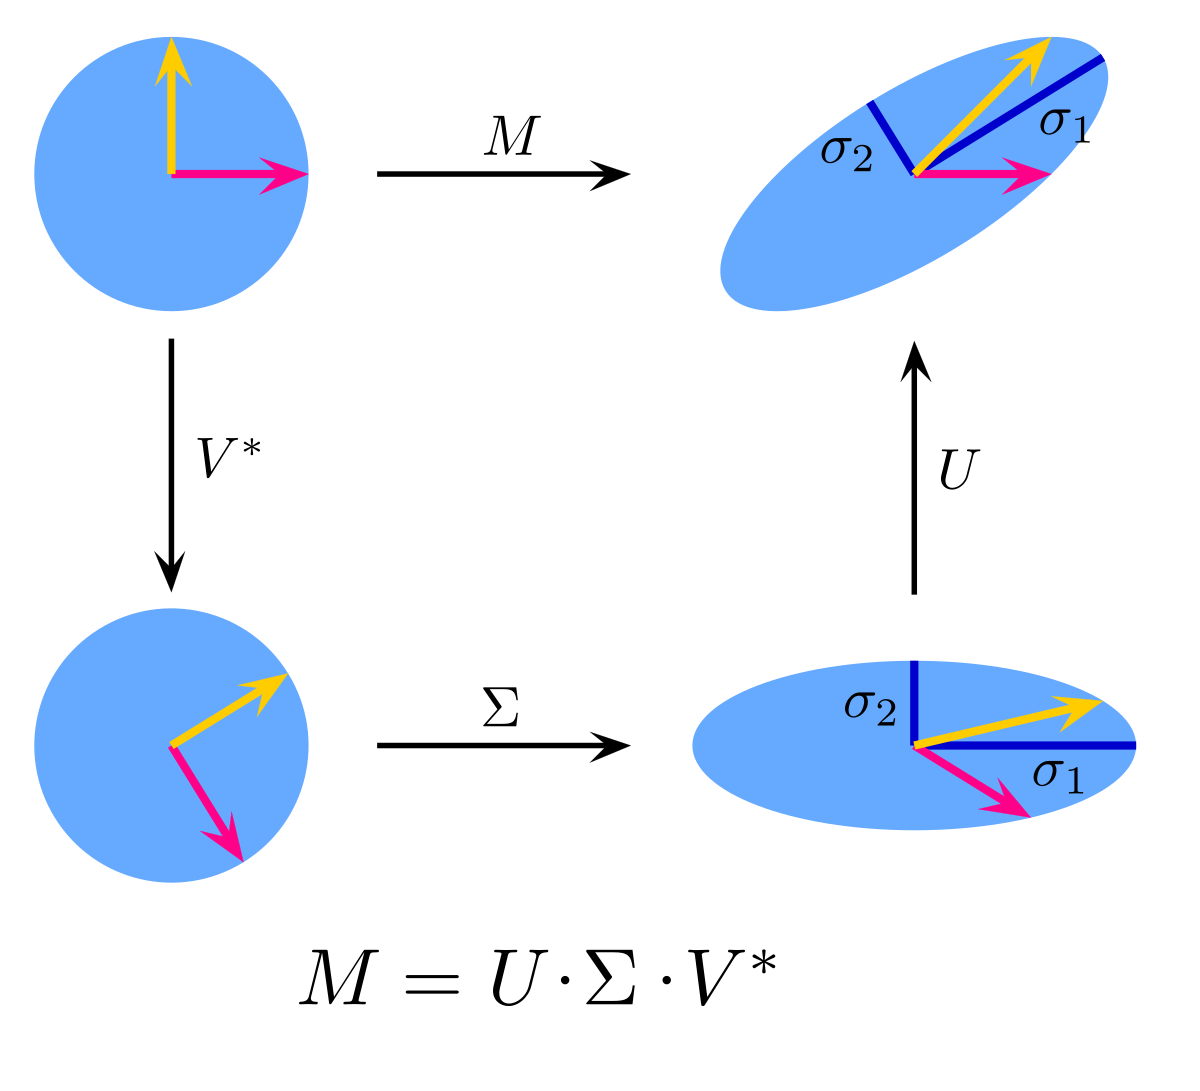
\includegraphics[width = 0.3\textwidth]{./figures/SVD.png}
  \caption{A diagram for Single Value Decomposition}
  \label{}
\end{figure}

More generally we map a unit sphere in $\R^n$ to the ellipsoid in $\R^m$. As the basis vectors are orthonormal we stretch in orthogonal directions.

\subsection{How to find the SVD}

Let us firstly look at $A^*A$, this matrix is semi-definite. Hence diagonalisable as it is self adjoint. It must have a basis of eigenvectors and all it's eigenvalues are non-negative.

\begin{align*}
  A^*A &= (U\Sigma V^*)U\Sigma V^*\\
  &= V^{**}\Sigma^*U^*U\Sigma V^*\\
  &= V\Sigma^TU^{-1}U\Sigma V^*\\
  &= V\Sigma^T\Sigma V^{-1}\\
\end{align*}
We can see that we have a square $n\times n$ matrix for $\Sigma^T\Sigma$. Then the whole matrix is diagonal, with the diagnonal of $\sigma_i$ up to $r$.
$$ \begin{pmatrix}
  \sigma_1^2 & & & & &\\
  & \sigma_2^2 & & & &\\
  &  & \sigma_2^2 & & &\\
  & & & \ddots & & & &\\
  & & & & \sigma_k^2 & &\\
  & & & & & \ddots & &\\
  & & & & & & 0 & \\
\end{pmatrix} $$

We can do a similar thing for $AA^*$, but we will get a $m\times m$ matrix.\\

\begin{enumerate}
  \item The non-zero singular values $\sigma_1, \dots, \sigma_r$ are obtained as the square roots of the non-zero eigenvalues $\l_1,\dots,\l_r$ of $A^*A$ or $AA^*$. That is, $\displaystyle{\sigma_i = \sqrt\l_i}$.
  \item The columns $\vec v_i$ of $V$ are an orthogonal basis of $\F^m$ consisting of eigenvectors of $A^*A$.
  \item The columns of $\vec u_i$ of $U$ are given by $\vec u_i = \frac{1}{\sigma_i}A\vec v_i$ and are an orthonormal basis of $\F^m$ consisting of eigenvectors of $AA^*$.
\end{enumerate}
The single values are unique, but the matrices $U$ and $V$ are not.


\end{document}
